\documentclass[output=collectionpaper]{langsci/langscibook}


\title{Gender in New Guinea}

\author{%
Erik Svärd
\affiliation{earlier Stockholm University}
}%


\abstract{%
\label{firstpage:Svaerd}
The present study classifies gender systems of 20 languages in the New Guinea region, an often neglected area in typological research, according to five criteria used by \citet{DiGarbo2014} for African languages. The results show that gender in New Guinea is diverse, although around half of the languages have two-gendered sex-based systems with semantic assignment, more than four gender-indexing targets, and no gender marking on nouns. The gender systems of New Guinea are remarkably representative of the world, although formal assignment is underrepresented. However, the gender systems of New Guinea and Africa are very different. The most significant difference is the prevalence of non-sex-based gender systems and gender marking on nouns in Africa, whereas the opposite is true in New Guinea. Finally, four typologically rare characteristics are singled out: (1) size and shape as important criteria of gender assignment, with large/long being masculine and small/short feminine, (2) the co-existence of two separate nominal classification systems, (3) no gender distinctions in pronouns, and (4) verbs as the most common indexing target.
\medskip

\textbf{Keywords:} agreement, grammatical gender, indexation, New Guinea, Papuan, typology.
}%

\maketitle
\begin{document}


\section{ Introduction and background}

Most typological research on gender has focused on languages in Eurasia, Africa, Australia, and the Americas. Less researched is the region of New Guinea containing as many as one sixth of all languages of the world. In recent descriptions languages of New Guinea of highly variable genealogical affiliation have been shown to exhibit many unusual gender systems. This is important for the study of gender as gender systems are often very stable and not prone to borrowing. However, little has been done to survey the diversity of gender in New Guinea. The purpose of this paper is to counteract this issue by investigating 20 New Guinean languages, both Papuan and non-Papuan, for which gender has been described and to compare their gender systems in an areal and a typological perspective. Specifically, the research questions are:

\begin{itemize}
\item How is grammatical gender expressed in a diverse sample of 20 languages of New Guinea?

\item How do the gender systems of New Guinea compare with other geographical areas (notably Africa) and the world as a whole?

\item Are there any phenomena in gender which are unique to or surprisingly common in the languages of New Guinea?
\end{itemize}


In order to investigate this, five criteria are used to classify the gender systems of New Guinea. The distribution of values of these criteria are then compared with the world in general and Africa in particular.

\subsection{ Defining gender}

\citet[231]{Hockett1958} defines gender as ``classes of nouns reflected in the behavior of associated words''. In other words, gender is conceived of as noun classes triggering agreement. The idea of gender as based on the behavior of associated words is reflected in the focus on agreement, which \citet[4]{Corbett1991} calls the determining criterion of gender. In order to define gender, Corbett presents Steele's (\citealt*{Steele1978}) description of agreement:

\begin{quote}
The term \textit{agreement} commonly refers to some systematic covariance between a semantic or formal property of one element and a formal property of another. For example, adjectives may take some formal indication of the number and gender of the noun they modify. \\
(\citealt[610]{Steele1978} as cited in \citealt[105]{Corbett1991})
\end{quote}

According to Corbett, agreement is an asymmetric relationship between the controller (i.e., the element determining agreement, e.g., subject noun phrase) and the target (i.e., the element whose form is determined by agreement) \citep[4]{Corbett2006}. Importantly, Corbett adopts a `canonical approach': that is, the basis for Corbett's discussion are those `canonical' instances which are best and clearest but not necessarily the most frequent \citep[9]{Corbett2006}. Canonical agreement can be summarized as follows (adapted from \citealt[9]{Corbett2006}):

\begin{itemize}
\item the controller is present, has overt expressions of features, and is consistent in agreement, and its part of speech is not relevant;
\item the target has bound expression of agreement, obligatory and regular marking which is doubling the marking of the noun, has a single controller, and its part of speech is not relevant;
\item the domain in which agreement occurs is local, and it is one of multiple domains.
\end{itemize}

More recently, \citet[8]{DiGarbo2014} gives a few examples illustrating the fact that in many languages both pronouns and noun phrase-internal targets do not presuppose a syntactic antecedent or controller. In order to counter this, \citet{DiGarbo2014} uses the term \textit{indexation} instead, following \citet{Croft2001,Croft2003,Croft2013} and \citet{Iemmolo2011}. In this definition, indexation is used to refer to grammatical strategies signaling (i) lexical and grammatical properties of nouns, and (ii) semantic properties of NP referents, which are independent of the presence of any overt syntactic antecedent (\citealt[8]{DiGarbo2014}). Following Di Garbo, the following terms are used in this study (adapted from \citealt[8]{DiGarbo2014}):

\begin{itemize}
\item \textit{indexing target} or \textit{index} refers to entities with inflectional morphology signaling gender;
\item \textit{syntactic antecedent} refers to the NP indexed by the pronominal target;
\item \textit{indexation trigger} or \textit{trigger} refers to the entities that activate the use of a certain indexation pattern in a given discourse domain.
\end{itemize}

Despite the difference in terminology, the end result of both agreement in \citet{Corbett1991} and indexation in \citet{DiGarbo2014} is the same, with both being cover terms for the same linguistic feature. Since this is mainly a typological study, its purpose is to be comparable with earlier and future typological research on gender without relying on theoretical concepts which are as yet not widely accepted. However, since indexation is gaining ground, it is embraced in this chapter.

\subsection{Gender research on New Guinea}

Although gender has not been extensively researched in New Guinea, the region shows much promise for exhibiting a high variety of gender systems. The New Guinea region is home to approximately 1,200 languages belonging to around three dozen language families spoken in an area smaller than 900,000 km\textsuperscript{2}, which makes it the most linguistically diverse region in the world \citep[357]{Foley2000}. Nevertheless, there are two dominating language families: the Austronesian family, spoken in the coastal areas, and the Trans New Guinean (TNG) family, which is concentrated to the mountainous inland. The Austronesian and the TNG languages comprise around 300 languages each and typically do not show gender, although there are some important exceptions (\citealt[358--363]{Foley2000}). Thus, gender is lacking at least in approximately half of the languages of New Guinea. As for the remaining languages, gender is found in the West Papuan, Sko, and Sepik languages, as well as several isolates such as Yava, Burmeso, and Kuot \citep[371]{Foley2000}.%
\footnote{\citet[371]{Foley2000} also mentions the Sulka language of New Britain, but there are no indications of a gender system in the grammar by \citet{Tharp1996}.} %
Gender is also present in Torricelli and Lower Sepik-Ramu languages, but as parts of larger and more complex systems of noun classification \citep[371]{Foley2000}. It also occurs in some isolated cases in the TNG family, such as Nalca (Mek) (\citealt{Svaerd2013}) and the Ok languages, e.g., Mian \citep{Fedden2011}, and in very few Austronesian languages, including Teop (Oceanic) (\citealt{Mosel2000}). By counting these gendered languages based on the numbers given by \citet{Foley2000}, gender in New Guinea can be estimated to occur in at least 120 languages of different families and isolates. The genealogical diversity suggests that gender may be highly diverse in New Guinea.

However, Foley suggest that gendered languages of New Guinea have some features in common, including the presence of gender assignment based on specific criteria of size and shape, as well as the presence of languages with two separate systems (\citealt{Foley2000}; \citealt[8--9]{Svaerd2015}). Combined with the observation that gender in New Guinea is concentrated in languages with high genealogical diversity, this suggests that gender may be highly diverse in New Guinea.

\section{Method and data}
\label{sec:Svard:2}

The sampling method used in this study is a \textit{variety sample} \citep{Bakker2012}. Rather than trying to represent the real population of languages as would be achieved by a probability sample, the sample is constructed such as to achieve the largest variety of results in regard to the chosen feature entirely omitting languages lacking the feature.


In this study, the sample is restricted to New Guinea as delimited by \citet[357]{Foley2000}, including New Guinea proper as well as surrounding islands. First and foremost, the sample includes only languages with gender. Secondly, the languages were chosen from as many families as possible, as far as the availability of material permits, while still accounting for variation within families if there were reasons to do so, primarily based on the information by \citet{Foley2000} and others.



\tabref{tab:Svard:1} lists the languages of the sample together with family, genus, ISO code, and source, together with a map of the languages shown in \figref{fig:Svard:1}. The names primarily follow Glottolog, except for Motuna (Glottolog: Siwai), where I follow \citet{Onishi1994}. Also, the Glottolog form Warapu is used despite Barupu occurring in \citet{Corris2005}. Furthermore, language families and genera are based on Glottolog, so that a genus in the table below does not always agree with the genus for the same language in \textit{WALS}.

\begin{table}[htb]
\footnotesize
\begin{tabularx}{\textwidth}{lXlX>{\raggedright\let\newline\\\arraybackslash\hspace{0pt}}X}
\lsptoprule

\bfseries Family & \bfseries Genus & \bfseries ISO & \bfseries Language & \bfseries Source\\
\midrule
Austronesian, Oceanic & Nehan-North Bougainville & tio & Teop & \citet{Mosel2000}\\
Isolate & – & gpn & Taiap & \citet{Kulick1992}\\
Isolate & – & bzu & Burmeso & \citet{Donohue2001}\\
Isolate & – & kto & Kuot & \citet{Lindstroem2002}\\
Left May & – & amm & Ama & \citet{Arsjoe1999}\\
Lower Sepik-Ramu & Lower Sepik & yee & Yimas & \citet{Foley1991}\\
Ndu & – & mle & Manambu & \citet{Aikhenvald2008}\\
North Bougainville & – & roo & Rotokas & \citet{Robinson2011}\\
Sepik & – & aau & Abau & \citet{Lock2011}\\
&  & sim & Mende & \citet{Hoel1994}\\
Sko & – & skv & Skou & \citet{Donohue2004}\\
&  & wra & Warapu/Barupu & \citet{Corris2005}\\
South Bougainville & – & siw & Motuna/Siwai & \citet{Onishi1994}\\
Torricelli & – & avt & Au & \citet{Scorza1985}\\
& Arapesh & ape & Bukiyip & \citet{Conrad1991}\\
& West Palai & van & Walman & \citet{Brown2008a}\\
Trans-New Guinea & Mek & nlc & Nalca & Svärd (2013); Wälchli (to appear)\\
& Ok-Oksapmin & mpt & Mian & \citet{Fedden2011}\\
&  & opm & Oksapmin & \citet{Loughnane2009}\\
West Papuan\footnotemark{} & – & ayz & Maybrat & \citet{Dol2007}\\
\lspbottomrule
\end{tabularx}

\caption{The language sample. The en dash indicates no grouping or that the language is itself the closest node to the family node.}
\label{tab:Svard:1}
\end{table}

\footnotetext{More recent studies suggest that the traditional West Papuan Phylum is probably not an accurate genealogical grouping, but instead consists of as many as seven unrelated language groups (\citealt[5]{Dol2007}). Since the exact position of Maybrat in such a regrouping is unknown to the present author, West Papuan is kept here as proxy to a genealogical family.}

\begin{figure}[htb]
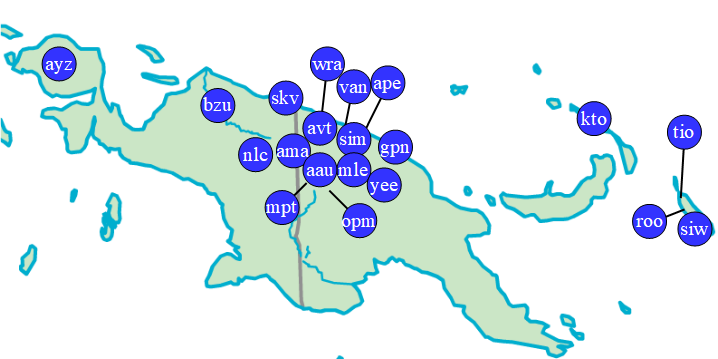
\includegraphics[width=\textwidth]{figures/09/Simple/fig1.png}
\caption{The geographical locations of the languages in the sample labeled with ISO codes}
\label{fig:Svard:1}
\end{figure}


The main sources of data used in this study are reference grammars, which are listed for each language in \tabref{tab:Svard:1} above. However, many descriptions do not mention the language as having a gender system if gender only occurs in pronouns, so it was also necessary to examine the sections on pronouns. If the available descriptions for a language neither mentioned gender nor showed it directly in the section(s) about pronouns or in glossed examples, the language was not considered as eligible for the sample.

In order to make the languages of the study typologically comparable, the study employs five classificatory criteria used by \citet{DiGarbo2014} to classify the gender systems of Africa, viz.,

\begin{itemize}
\item Sex-based and non-sex-based gender systems.
\item Number of genders.
\item Gender assignment.
\item Number of gender-indexing targets.
\item Occurrence of gender marking on nouns.
\end{itemize}


Di Garbo also uses other classificatory criteria in order to investigate the interactions of gender and number, and gender and evaluative morphology. However, this study is not aimed to directly investigate these interactions, and thus only the criteria above were chosen.


An important advantage of adopting Di Garbo's approach is that this makes the results for New Guinea directly comparable with Africa as for the selected criteria. In addition, since the first three criteria are the same as the ones used in the \textit{WALS} chapters by Corbett (\citealt{Corbett2013,Corbett2013a,Corbett2013b}), much of the results is comparable to a worldwide sample. In order to illustrate the distributions, maps were created using the Interactive Reference Tool of the \textit{World atlas of language structures} (\textit{WALS})\footnote{See http://www.eva.mpg.de/lingua/research/tool.php.} using ISO codes and coordinates from Glottolog.

\section{ Overview of gender characteristics}
\label{sec:Svard:3}

In the following sections, the distribution of values of the criteria mentioned in \sectref{sec:Svard:3} are presented and discussed. Each criterion is discussed with the values shown in a table, followed by some examples of the feature in the sample. In \sectref{sec:Svard:4}, these results are discussed from a typological perspective.

It is important to point out that five languages of the sample were found to have two separate systems of noun classification. As will be discussed in \sectref{sec:Svard:5.2}, only Burmeso exhibits two equivalent gender systems, whereas the other four rather distinguish between gender and noun classifiers. For this reason, the two gender systems of Burmeso will be combined for the purpose of comparison in this chapter, although the values assigned to the separate systems will be given in parenthesis whenever applicable.

\subsection{ Sex-based and non-sex-based gender systems}
\label{sec:Svard:3.1}

Following \citet[62]{DiGarbo2014}, each gender system is classified as either sex-based or non-sex-based based according to the typology by \citet{Corbett2013b}. Sex-based are those where the gender assignment is based at least partly on natural gender, which often surfaces as masculine-feminine distinctions. Consequently, non-sex-based gender systems are those where gender is not based on natural gender. However, according to \citet{Corbett2013b}, all non-sex-based systems are based on some notion of animacy.

As shown in \tabref{tab:Svard:2} and \figref{fig:Svard:2}, sex-based systems are by far the most common ones, with 19 of 20 languages having natural gender as their semantic core. Only the sole Austronesian language Teop exhibits a non-sex-based system.

\begin{table}

\begin{tabularx}{\textwidth}{XXXX}
\lsptoprule

\bfseries Sex-based or non-sex-based & \bfseries No. of lgs. & \bfseries \% & \bfseries Language\\
\midrule
Sex-based & 19 & 95\% & {Abau}

{Ama}

{Au}

{Bukiyip}

{Burmeso}

{Kuot}

{Manambu}

{Maybrat}

{Mende}

{Mian}

{Motuna}

{Nalca}

{Oksapmin}

{Rotokas}

{Skou}

{Taiap}

{Walman}

{Warapu}

Yimas\\
Non-sex-based & 1 & 5\% & Teop\\
\midrule
Total: & 20 & 100\% & \\
\lspbottomrule
\end{tabularx}
\caption{Sex-based and non-sex-based gender systems in the sample}
\label{tab:Svard:2}
\end{table}

\begin{figure}
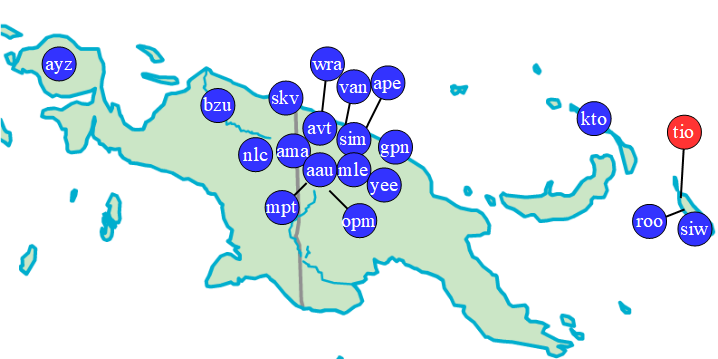
\includegraphics[width=\textwidth]{figures/09/Simple/fig2.png}
\caption{Sex-based and non-sex-based systems. Colors indicate: sex-based (blue) and non-sex-based (red).}
\label{fig:Svard:2}
\end{figure}


Sex-based gender systems present some difficulty in assigning nouns denoting inanimate referents. Non-sex-based systems, i.e., systems based on animacy, can potentially assign every noun according to animacy alone. However, sex-based systems do not by definition have any specific way of assigning nouns that refer to objects without natural gender. Thus, based on how inanimate nouns are assigned gender, the sex-based gender systems in the sample can be further divided into three groups where inanimates are assigned to

\begin{enumerate}
\item one of the sex-based genders,
\item both of the sex-based genders based on other criteria, or
\item one or more other non-sex-based genders.
\end{enumerate}


As will be discussed in \sectref{sec:Svard:3.2}, almost half of the languages in the sample (9 of 20) have only two genders, both of which are sex-based. Thus, since option 3 is only available in languages with more than two genders, almost half of the languages in the sample assign inanimate nouns to one of the sex-based genders.

Assigning inanimates to only one of the two genders occurs e.g., in Mende (Sepik), where gender is distinguished only in second and third person singular pronouns. For animate referents, the form of the pronoun is determined by the sex of the referent, while inanimates are usually referred to with the feminine forms (\citealt[17]{Hoel1994}). An example of this is shown in (\ref{ex:Svard:1}), where \textit{Max} (male name) (\ref{ex:Svard:1}a) and \textit{Lusi} (female name) (\ref{ex:Svard:1}b) occur with the masculine and feminine pronoun forms respectively, and the inanimate \textit{masiji} `hair' (\ref{ex:Svard:1}c) is referred to with the feminine form. Mende has thus a distinction masculine vs.\ other.

\ea
\label{ex:Svard:1}
Mende (Sepik) (\citealt[19, 31, 46]{Hoel1994})\\
\begin{xlist}
\ex
\gll Max wasilaka ri-a\\
     M. big 3\textsc{sg.m-inten}\\
\glt ``Max is big.''

\ex
\gll Lusi kava awu-n u-nda sir-a\\
     L. {bad\footnotemark} fight\textsc{{}-obj} do\textsc{{}-hab} \textsc{3sg.f-inten}\\
\glt ``Lusi is a good fighter.''

\ex
\gll masiji-n tivi unak si horngo-ku-a\\
     hair-\textsc{obj} tie so.that.not 3\textsc{sg.f} loosen-\textsc{fut-inten}\\
\glt ``Tie the hair so that it won't loosen.''
\end{xlist}
\z
\footnotetext{When used with the habitual -\textit{nda}, \textit{kava} `bad' functions as an intensifier (Hoel et al. 1994:31).}


Assigning inanimates to both sex-based genders based on other criteria is more common in the sample. In most languages, the assignment of inanimates is based on semantic criteria, most commonly on the criteria shape and size (see also \sectref{sec:Svard:5.1} below). One such a language is Abau (Sepik), where three-dimensional or long or extended objects, as well as liquids are masculine, whereas two-dimensional, flat or round objects with little height as well as abstract entities are feminine \citep[47]{Lock2011}. Thus, \textit{su} `coconut' (round), \textit{now} `tree' (long), and \textit{hu} `water' (liquid) are masculine, while \textit{iha} `hand' (flat) and \textit{hne} `bird's nest' (round with little height) are feminine (\citealt[48--50]{Lock2011}). In a language such as Abau, this is very much based on the speaker's perception. This can be seen in (\ref{ex:Svard:2}); when referring to the tree from which he makes the paddle (\ref{ex:Svard:2}a), \textit{youk} `paddle' is masculine, since the tree is long and not at all round or flat. However, when referring to the actual paddle (\ref{ex:Svard:2}a), which has the salient features of flat and round, the feminine form is used.


\ea
\label{ex:Svard:2}
Abau (Sepik) \citep[50]{Lock2011}\\
\begin{xlist}
\ex
\gll Ha-kwe youk se seyr.\\
     \textsc{1sg.sbj-top} paddle \textsc{3sg.m.obj} cut\\
\glt ``I cut the `paddle' tree.''
\ex
\gll Ha-kwe youk ke lira.\\
     \textsc{1sg.sbj-top} paddle \textsc{3sg.f.obj} see\\
\glt `I see the paddle.'
\end{xlist}
\z

The third type of sex-based systems is one where inanimates are assigned to genders other than sex-based ones. Naturally, this can only occur in languages with more than two genders. An example of a language with such a system is Nalca (TNG, Mek) (\citealt{Svaerd2013}; \citealt{Waelchli2018}). Nalca has five main genders: masculine, feminine, neuter, default, and non-noun. As shown in (\ref{ex:Svard:3}), these are apparent in a set of case marker hosts following the NP, which constitute the only indexing target in Nalca. The masculine and feminine genders are used exclusively for nouns denoting male and female humans respectively. Inanimates are divided between the neuter and default genders: the neuter contains all nouns of the phonological structure (C)V (including at least one noun denoting humans, \textit{me} `son, child'), while most inanimate nouns belong to the residual default gender. The default gender also contains some gender-neutral nouns denoting humans, most of which are plural, e.g., \textit{nang} `people'. The non-noun gender is used e.g., with adverbs, locatives, and despite its name the nominalizer \textit{-a'}. It is also used when gender is switched off, in which case nouns still trigger agreement but due to syntactic phenomena agree with the non-noun gender.%
\footnote{The concept of switching gender on and off is an extremely rare phenomenon and goes well beyond the bounds of this study. For a comprehensive description of the Nalca gender system and discussion on switching gender on and off, see \citet{Waelchli2018}.} %
In the examples below, both the neuter \textit{si} `name' and the masculine name \textit{Zakheus} `Zacchaeus' are shown in (\ref{ex:Svard:3}a), the feminine \textit{genong} `mother' in (\ref{ex:Svard:3}b), the default (\textsc{default)} \textit{pik} `way' in (\ref{ex:Svard:3}c), and the two non-noun (\textsc{nnoun}) constructions in (\ref{ex:Svard:3}d). The first instance of non-noun gender in (\ref{ex:Svard:3}d) is due to the intervention of the quantifier \textit{nauba} `many' between \textit{nimi} `men', which belongs to default gender, and the case marker host, whereas the second is due to the nominalizer \textit{-a'}.


\ea
\label{ex:Svard:3}
Nalca (TNG, Mek) (own examples)\\
\begin{xlist}
\ex
\gll alja si ne-ra Zakheus be-k u-lu{}-m-ok\\
     \textsc{3sg.gen} name \textsc{n-top} Z. \textsc{m-abs} be-\textsc{i}\textsc{pfv-pst.3sg}\\
\glt `a man called by name Zacchaeus' (Lk 19:2)\footnotemark{}\\
lit. `his name was Zacchaeus'

\ex
\gll Nadya genong ge-ra heknya do?\\
     \textsc{1sg.gen} mother \textsc{f-top} who \textsc{q}\\
\glt `Who is my mother?' (Mk 12:48)

\ex
\gll Na bi-nim-na pik e-ra ugun-da ella u-lu-lum …\\
     \textsc{1sg} go-\textsc{fut-prs.1sg} way \textsc{default-top} \textsc{2pl-top} knowledge be-\textsc{ipfv-prs.2pl} {}\\
\glt `And you know the way where I am going.' (Jn 14:4)

\ex
\gll {\ldots} nimi nauba a-ra seleb longo-m-ek-a' a-k eib-ok\\
    {} men many \textsc{nnoun-top} already assemble-\textsc{prf-pst.3pl-nmlz} \textsc{nnoun-abs} see[\textsc{pfv}]\textsc{{}-pst.3sg}\\
\glt `… he saw the large crowds…' (Mt 6:34)\\
lit. `he saw that many men had assembled'
\end{xlist}
\z
\footnotetext{The overwhelming majority of data available in Nalca consists of a translation of the New Testament. The English translation used is the American Standard Version, whereas the glossings and literal translations were devised by the present author. For a description and discussion of the methodology, see Svärd (2013) and Wälchli (to appear).}

Finally, the only non-sex-based gender systems in the sample occurs in the Austronesian language Teop, which has two genders (I and II) with two subgenders for the first gender (I-E and I-A, reflecting the form of the singular article preceding nouns. The genders and the nouns that belong to them are:

\begin{itemize}
\item \textit{Gender I-E}: Contains all proper names, kinship terms, and nouns denoting pets or humans with a particular communal or important social status (\citealt[334--335]{Mosel2000}).

\item \textit{Gender I-A:} Contains most nouns and can be considered the unmarked gender (\citealt[336--338]{Mosel2000}).

\item \textit{Gender II:} Contains names of plants and their parts (but not fruits), objects made of plant material, invertebrates without legs, and many mass and abstract nouns (\citealt[338]{Mosel2000}).
\end{itemize}

This is strikingly similar to the noun classification system found in Siar (\citealt{Frowein2011}; not in the sample), spoken on the opposite coast. Siar does not have a true gender system, since it only shows gender on articles preceding nouns and thus does not exhibit indexation.%
\footnote{In this study, a word is only considered an indexing target if it has a functional load other than expressing gender and number. The reason for this is that otherwise languages such as Siar, which has a set of markers preceding only nouns, would be considered as having gender. Such a system would be difficult to separate from a system showing noun classification only on the noun itself, i.e., without indexation.} %
However, nouns are still assigned according to a system of nominal classification similar to Teop:

\begin{itemize}
\item \textit{Proper}: Contains mostly names, kinship terms and other nouns closely related to humans and culture such as professions (\citealt[104--105]{Frowein2011}).

\item \textit{Common 1}: A very heterogenous residual class, consisting of all nouns not in the proper or common 2 genders \citep[108]{Frowein2011}.

\item \textit{Common 2}: Contains semantically marked nouns, including entities that are smallish or individuated from a greater mass, but also other semantic types; some examples are insect, birds, other smallish animals, plants and parts of plants, tools, loanwords, geographic locations, some meteorological phenomena, groups and sets, and ordinals (\citealt[105--107]{Frowein2011}).
\end{itemize}

Teop and Siar thus clearly display the differences between a gender system and a simpler noun classification system according to the criteria of gender used in this paper.

\subsection{ Number of genders}
\label{sec:Svard:3.2}

The second criteria concerns the number of genders in a language, based on \citet{Corbett2013}. Each language is assigned the value two, three, four, or five or more genders (see \tabref{tab:Svard:3} and \figref{fig:Svard:3}). The majority of the languages have only two genders, in all cases sex-based. Only one, Mian, has four genders. Of the remaining languages, three languages have three genders, whereas the remaining five languages have five or more genders, viz., Nalca (5), Motuna (6), Burmeso (9 > 3/6),%
\footnote{Burmeso has two gender systems, with three genders belonging to the first system and the other six belonging to the second system (see \sectref{sec:Svard:5.2}).} %
Yimas (around 12), and Bukiyip (18 genders).

\begin{table}
\begin{tabularx}{\textwidth}{XXXX}
\lsptoprule

Number of genders & No. of lgs. & \% & Languages\\
\midrule
Two & 11 & 55\% & {Abau}

{Kuot}

{Manambu}

{Maybrat}

{Mende}

{Oksapmin}

{Skou}

{Taiap}

{Teop}

{Walman}

Warapu\\
Three & 3 & 15\% & {Ama}

{Au}

Rotokas\\
Four & 1 & 5\% & Mian\\
Five or more & 5 & 25\% & {Nalca (5)}

{Motuna (6)\footnotemark{}}

{Burmeso (9 → 3/6)\footnotemark{}}

{Yimas ({\textasciitilde}12)}

Bukiyip (18)\\
\midrule
Total: & 20 & 100\% & \\
\lspbottomrule
\end{tabularx}
\caption{Number of genders in the languages of the sample}
\label{tab:Svard:3}
\end{table}


%\addtocounter{footnote}{-2}
%\stepcounter{footnote}
\footnotetext{\citet{Onishi1994} states that Motuna has six genders: masculine, feminine, diminutive, local, manner, and dual-paucal. However, the author does not elaborate on gender assignment, and I have been unable to satisfactorily conclude that the dual-paucal is truly a gender, which Onishi states. However, all form a complementary and mutually exclusive system, with separate identifiable markers and where a word may take only one gender.}
%\stepcounter{footnote}
\footnotetext{Burmeso has nine genders in total: three belong to the first gender system, whereas six belong to the second.}

\begin{figure}
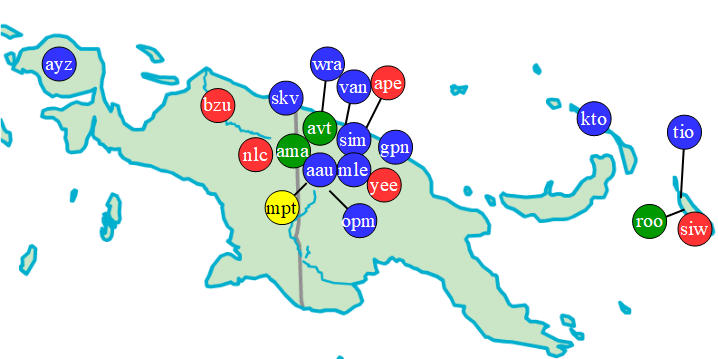
\includegraphics[width=\textwidth]{figures/09/Simple/fig3.png}
\caption{Number of genders. Colors indicate: two (blue), three (green), four (yellow), and five or more (red).}
\label{fig:Svard:3}
\end{figure}



In contrast to the previous criterion, it is more difficult to identify subgroups based on values of the number of genders; e.g., the languages with three genders are very different from each other. Nevertheless, some of the languages have the following specific characteristics of

\begin{enumerate}
\item two genders where one is unmarked,
\item three genders consisting of masculine, feminine, and neuter, or
\item very large systems.
\end{enumerate}

More than half of the languages with two genders have one which is unmarked, all of which are sex-based. Consequently, in these languages, either the feminine or the masculine gender is unmarked. An example of such a language is Maybrat (West Papuan), which has the conveniently named genders masculine and unmarked (i.e., non-masculine) \citep[89]{Dol2007}. Thus, nouns denoting male humans (or in some cases other male animates) are masculine, whereas all others (including those denoting females) belong to the unmarked gender. This is shown in (\ref{ex:Svard:4}). In (\ref{ex:Svard:4}a) `old' indexes `his father', in (\ref{ex:Svard:4}b) `his mother', and in (\ref{ex:Svard:4}c) `big' indexes `house'.

\ea
\label{ex:Svard:4}
Maybrat (West Papuan) \citep[90]{Dol2007}\\
\begin{xlist}
\ex
\gll y-atia \textbf{y}{}-anes\\
     \textsc{3m-}father \textsc{\textbf{3m}}{}-old\\
\glt `His father is old.'/`his old father'
\ex
\gll y-me \textbf{m}{}-anes\\
     \textsc{3m-}mother \textsc{\textbf{3u}}{}-old\\
\glt `His mother is old.'/`his old mother'
\ex
\gll amah \textbf{m}{}-api\\
     house \textsc{\textbf{3u}}{}-big\\
\glt `The house is big.'/`the big house'
\end{xlist}
\z

However, not all such languages use the masculine gender as the marked one. Languages where the masculine is marked are Warapu (Sko), Maybrat (West Papuan), Mende (Sepik), and Taiap (isolate), whereas the feminine is marked in Skou (Sko). It is also marked in Ama (Left May), which has three genders: masculine, feminine, and compound. However, the situation is more complex in Ama, both because there are three genders, and because the feminine also includes e.g., some non-female animates (\citealt[68]{Arsjoe1999}).

Except for Ama, which is mentioned above, the three-gendered systems belong to the second type, since all have masculine, feminine, and neuter. While this implies that inanimates are found only in the neuter gender, all languages assign some inanimates to the masculine and feminine genders as well, with or without sex-based motivation. For example, in Rotokas (North Bougainville), inanimate objects associated with male culture (such as hunting or warfare) and long, thin objects are masculine (see also \sectref{sec:Svard:5.1}), whereas most inanimates are assigned either to the feminine or to the neuter genders (\citealt[46--48]{Robinson2011}).

The third and final type is languages with very large gender systems, viz., Bukiyip (Torricelli, Arapesh) and Yimas (Lower Sepik-Ramu, Lower Sepik). These are markedly different from all other languages in the sample. The most immediate difference is of course the vastly larger number of genders. Bukiyip has as many as 18 genders (\citealt[8--10]{Conrad1991}), while Yimas has around a dozen genders, with \citet[119]{Foley1991} distinguishing 10 and \citet[175]{Phillips1993} as many as 16. All other languages in the sample have six genders or fewer. The Bukiyip genders and their indexing forms are shown in \tabref{tab:Svard:11} in \sectref{sec:Svard:3.5}. The most important feature of these two gender systems is that both have semantic-formal assignment and gender marking on nouns. These two factors, which are uncommon in the sample, are undoubtedly related to the subsistence of their large systems.

Finally, a highly interesting case is Burmeso, which is the only language in the sample with two gender systems. The first system has three genders (masculine, feminine, and neuter), each with an additional subgender for inanimates, whereas the second system has six genders (I--VI). The exact nature of the gender systems and their interaction will be discussed further in \sectref{sec:Svard:5.2}.

\subsection{Gender assignment}
\label{sec:Svard:3.3}

The third criterion concerns gender assignment and contains two values (see \tabref{tab:Svard:4} and \figref{fig:Svard:4}), viz., semantic, or semantic and formal.


%%please move \begin{table} just above \begin{tabular
\begin{table}
\begin{tabularx}{\textwidth}{XXXX}
\lsptoprule

Gender assignment & No. of lgs. & \% & Language\\
\midrule
Semantic & 16 & 80\% & {Abau}

{Ama}

{Au}

{Burmeso}

{Manambu}

{Maybrat}

{Mende}

{Mian}

{Motuna}

{Oksapmin}

{Rotokas}

{Skou}

{Taiap}

{Teop}

{Walman}

Warapu\\
Semantic and formal & 4 & 20\% & {Bukiyip}

{Kuot}

{Nalca}

Yimas\\
\midrule
Total: & 20 & 100\% & \\
\lspbottomrule
\end{tabularx}

\caption{Systems of gender assignment in the sample}
\label{tab:Svard:4}
\end{table}

\begin{figure}[htb]
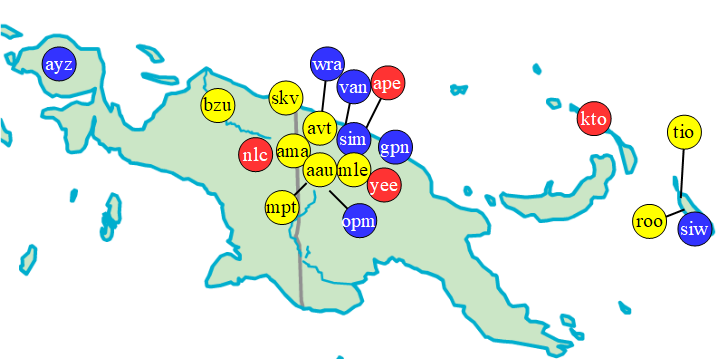
\includegraphics[width=\textwidth]{figures/09/Simple/fig4.png}
\caption{Systems of gender assignment. Colors indicate transparent semantic (blue), semantic and formal (red), and semantic and opaque (yellow).}
\label{fig:Svard:4}
\end{figure}


As can be seen in \figref{fig:Svard:4}, the majority of languages in the sample have semantic assignment. However, there are major differences between the various semantic systems as to their complexity. As mentioned in \sectref{sec:Svard:3.1}, Mende (Sepik) has an extremely simple system of gender assignment, where all nouns denoting human or sometimes animate males are masculine while all other nouns are feminine.

In Rotokas (North Bougainville), however, the situation is more complex. Rotokas has three genders: masculine, feminine, and neuter. Both the masculine and the feminine gender contain nouns denoting male and female referents respectively, but complexity arises for inanimates. The masculine gender contains many inanimate objects, which are often associated with male culture or which are long or thin \citep[46]{Robinson2011}. The feminine gender also contains many inanimate objects, some of which are tools or related to water, but many which have no apparent semantic or formal criteria at all \citep[47]{Robinson2011}. Finally, as expected, many inanimate nouns belong to the neuter gender \citep[48]{Robinson2011}.


Thus, while a learner of Mende is easily able to guess the correct gender of any noun, a learner of Rotokas is hard-pressed to guess the correct gender of an inanimate object. Even if there are rules, many of these are probably not tacitly known. Furthermore, even if the rules for gender assignment can be explicitly stated, the system may still be opaque if the rules are not general or have numerous exceptions. One example is Manambu (described further below), where gender assignment sometimes carries the notion of large size, so that larger animals are masculine and smaller animals feminine. However, insects are masculine despite their small size.%
\footnote{It is of course possible to imagine various explanations why insects are not feminine, e.g., perhaps are they are not regarded as animals. However, this only further illustrates the reason for not regarding Manambu gender assignment as transparent. Although there certainly is a general pattern of size distinctions for gender assignment in Manambu, it is merely a pattern and not a rule.}

It is therefore possible to further split the systems with semantic assignment into two: transparent semantic vs.\ semantic + opaque (\figref{fig:Svard:5}), where opacity signals the inability of the researcher to find any clear semantic or formal criteria for gender assignment. It is possible that a language may have semantic + formal + opaque assignment, but no such system was clearly identified in the sample. This thus gives rise to three types of gender assignment: transparent semantic, semantic and formal, and semantic and opaque (\tabref{tab:Svard:5}).

\begin{table}
\begin{tabularx}{\textwidth}{XXXX}
\lsptoprule

Gender assignment & No. of lgs. & \% & Language\\
\midrule
Transparent semantic & 8 & 40\% & Au\footnotemark{}

Maybrat

Mende

Motuna

Oksapmin

Taiap

Walman

Warapu\\
Semantic and formal & 4 & 20\% & {Bukiyip}

{Kuot}

{Nalca}

Yimas\\
Semantic and opaque &  8 & 40 & Abau

Ama

Burmeso

Manambu

Mian

Rotokas

Skou

Teop\\
\midrule
Total: & 20 & 100\%  & \\
\lspbottomrule
\end{tabularx}
\caption{Types of semantic assignment of gender assignment in the sample}
\label{tab:Svard:5}
\end{table}

\footnotetext{It is not explicitly stated, but Au \citep{Scorza1985} appears to have a simple semantic system where nouns denoting human males are masculine, human females are feminine, and the rest are neuter. However, this is complicated somewhat by masculine and neuter agreement being homophonous in the singular.}


Since all languages have some form of semantic assignment, the most basic system is necessarily one where all nouns are assigned their genders based on few and clear semantic criteria. Mende has already been mentioned above and is exemplified in (\ref{ex:Svard:1}) in \sectref{sec:Svard:3.1}. However, semantic systems can be more complex while still retaining transparent semantic criteria, e.g., via a larger number of gender distinctions. One example is Motuna (South Bougainville), which has six genders: masculine, feminine, diminutive, local, manner, and dual-paucal (\citealt[68--69]{Onishi1994}). The forms of gender indexation in Motuna in are shown in Table~\ref{tab:Svard:6}.

%%please move the includegraphics inside the {figure} environment
%%\includegraphics[width=\textwidth]{GenderNewGuineaRevisedv4-img12.png}

\begin{table}
\small
\begin{tabularx}{\textwidth}{X>{\itshape}X>{\itshape}X>{\itshape}X>{\itshape}X>{\itshape}X}
\lsptoprule
& \normalfont Demon\-strative & \normalfont Article  & \normalfont Adjective/\newline classifier/\newline kinship term endings & \normalfont Possessor/\newline local NP endings  &  \normalfont Verbal endings \\
\midrule
Masculine &  ong & hoo/shoo  & -ng  & -ng  & -ng \\
Feminine & ana  & tii  & -na  & -na  & -na \\
Diminutive & oi  & tii  & -ni  & -ni  & -ni \\
Local & owo  & ti  & --  & -no  & -no \\
Manner & --  & tiwo  & --  & --  & -nowo \\
Dual-paucal & oi & tii & -- & -ni & -(n)i \\
\lspbottomrule
\end{tabularx}
\caption{Gender indexation forms in Motuna (adapted from \citealt[70]{Onishi1994})}
\label{tab:Svard:6}
\end{table}

In Motuna, animate referents are assigned gender based on their natural gender; this also includes nouns associated with mythical characters such as \textit{raa} `the sun' and \textit{hingjoo} `the moon', which are assigned the gender of their character (\citealt[70]{Onishi1994}). Animals are most commonly masculine, but can be assigned the feminine gender if emphasizing that the referent is a female. On the other hand, the majority of inanimate nouns are masculine, but can be treated as diminutive when emphasis is placed on their small size. This includes nouns which signify smallish things, e.g., \textit{irihwa} `finger' or \textit{kaa'} `young tree' (\citealt[71]{Onishi1994}). Nouns with spatial or temporal meaning are inherently local gender. The manner gender contains only two nouns. Finally, the dual-paucal gender can be used also when the speaker does not want to specify the gender of a sentential topic (\citealt[71]{Onishi1994}).

In contrast to the transparent semantic criteria in Mende and Motuna above, many languages have much more complex systems. If gender assignment is neither semantically transparent nor apparently formal, it is classified as being opaque, with Rotokas having already been mentioned at the beginning of this section. Another example of such a language is Manambu (Ndu), which exhibits the fairly common feature of gender assignment based on size and shape (see \sectref{sec:Svard:5.1}). Manambu has two genders, masculine and feminine, and in general gender assignment appears to follow semantic criteria. However, these are far from transparent:

\begin{enumerate}
\item Humans are assigned gender based on their sex, except nouns denoting small children, which can be assigned gender based on size (\citealt[116--117]{Aikhenvald2008}).
\item Higher animates are assigned based on their size and natural gender: larger animals are masculine, whereas smaller animals are feminine, except when the sex of the referent is known. Furthermore, nouns denoting young animals are feminine (\citealt[117]{Aikhenvald2008}).
\item Lower animates such as insects are masculine. However, if the lower animate has a certain shape, it is assigned gender based on shape; thus, \textit{gwa:s} `turtle' is feminine, since it is round, while \textit{mu} `crocodile' is masculine since it is long (\citealt[117]{Aikhenvald2008}).
\item Inanimates are assigned gender based on their size and shape: long and/or large objects are masculine, whereas small and/or round objects are feminine. Thus, \textit{vœy} `spear' is masculine, since it is large, but it is feminine if referring to small spears or shotguns (\citealt[117]{Aikhenvald2008}).
\item Natural phenomena are assigned gender based on whether they are complete or not: if they are uncompleted or if completeness is not emphasized, they are feminine; otherwise, they are masculine (\citealt[118]{Aikhenvald2008}). Thus, \textit{ga:n} `night' is feminine, unless it implies complete darkness, as is \textit{gәl} `cloud' if there are only a few but masculine if they cover the whole sky. Other natural phenomena are assigned gender based on their shape: e.g., `rainbow' is masculine since it is long, whereas `sun' is feminine since it is round; unless it is really hot, in which case it becomes masculine to reflect its intensity (\citealt[119]{Aikhenvald2008}).
\item Mass nouns and nouns covering `extent' follow complex patterns. In general, they are assigned gender based on extremity, so that smaller quantities are feminine, whereas larger quantities are masculine (\citealt[119--120]{Aikhenvald2008}). However, nouns denoting manner, language or voice, or time span are feminine; except for \textit{nabi} `year', which is masculine because it is very long (\citealt[119]{Aikhenvald2008}).
\end{enumerate}

There are in fact further assignment rules, but the important point is that rules of gender assignment are not semantically transparent. It is especially important to note that it is difficult to ascertain whether there are any rules or merely patterns. That is not to belittle the observations or to claim that the researcher, in this case Aikhenvald, has made anything wrong. Instead it illustrates the difference to transparent semantic systems, where all gender assignment rules are easily identifiable and apply to all nouns, whereas in opaque systems there are certainly some patterns that can be identified, but exceptions abound.

While it is easy to become amused by the seemingly arbitrary gender assignment rules, one important thing should be noted. In a language such as Manambu, gender has a very important pragmatic function, since it is available as a tool for the speaker to use when emphasizing certain features, not least in jokes:

\begin{quote}
As a joke, a man can be referred to with feminine gender, and a woman with masculine gender, depending on their `shape' and `size'. A smallish fat woman-like man can be treated as feminine, e.g.\ \textit{numa du} (big.\textsc{fsg} man) `fat round man'. And a largish woman can be ironically referred to with a masculine gender form, e.g.\ \textit{kә-dә numa-dә ta:kw} (\textsc{dem.prox-m.sg} big-\textsc{m.sg} woman) `this (unusually) big woman'. (\citealt[121]{Aikhenvald2008})
\end{quote}

The final category consists of the four languages with both semantic and formal assignment: Nalca is skewed towards semantic assignment, Kuot applies semantic and formal assignment roughly equally, and Bukiyip and Yimas favor formal assignment. For example, among the five genders in Nalca (see \sectref{sec:Svard:3.1} above), only the neuter is formal, but very much so since it contains only (but all) nouns of the phonological structure (C)V (\citealt{Waelchli2018}). In comparison, only three of the 18 genders in Bukiyip (see Table \ref{tab:Svard:10}) are semantic (masculine, feminine, and mixed or unspecified), whereas all others are morphological (\citealt[8]{Conrad1991}). The same is true for Yimas, where three genders are semantic, while the others are based on phonological criteria (\citealt[119]{Foley1991}).

\subsection{Number of gender-indexing targets}
\label{sec:Svard:3.4}

Following \citet[66]{DiGarbo2014}, the number of gender-indexing targets is given the value of one, two, three, or four or more. The results are shown in Table \ref{tab:Svard:6} and Figure \ref{fig:Svard:5}, while each type of indexing target is shown in Table \ref{tab:Svard:7}. The identification and counting of gender-indexing targets was based on the general guidelines used by \citet[66]{DiGarbo2014}, where the following general categories were used to identify targets: pronouns, adjectives, demonstratives, verbs, numerals, copulas, complementizers, and adpositions. However, no detailed analysis has been made of different subtypes of these groupings, so the results should be understood only as showing general patterns.


\begin{table}
\begin{tabularx}{\textwidth}{XXXX}
\lsptoprule
Number of gender-indexing targets & No. of lgs. & \% & Languages \\
\midrule
One & 4& 20\% & Ama

Mende

Nalca

Oksapmin\\

Two & 4 & 20\% & Warapu

Burmeso

Skou

Teop \\
Three & 2 & 10\% & Au

Taiap\\
Four or more & 10 & 50\% & Abau

Bukiyip

Kuot

Maybrat

Manambu

Mian

Motuna

Rotokas

Walman

Yimas\\
\midrule
Total: & 20 & 100\% \\
\lspbottomrule
\end{tabularx}
\caption{Number of gender-indexing targets in the languages in the sample}
\label{tab:Svard:7}
\end{table}

\begin{figure}
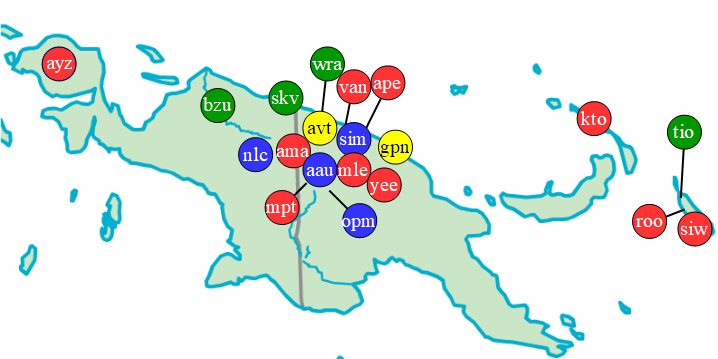
\includegraphics[width=\textwidth]{figures/09/Simple/fig5_new.png}
\caption{Number of gender-indexing targets. Colors indicate: one (blue), two (green), three (yellow), and four or more (red).}
\label{fig:Svard:5}
\end{figure}


\begin{table}
\small
\begin{tabular}{lp{.5cm}p{.5cm}p{.5cm}p{.5cm}p{.5cm}p{.5cm}p{1cm}}
\lsptoprule
Language & \rotatebox{45}{Pronouns\footnotemark{}} & \rotatebox{45}{Verbs} & \rotatebox{45}{Demonstratives} & \rotatebox{45}{Adjectives} & \rotatebox{45}{Numerals} & \rotatebox{45}{Prepositions} & \rotatebox{45}{Case hosts} \\
\midrule
Abau & W &  & X  &  & X &  & X \\
Ama &  & X  &  &  &  &  & \\
Au & X & X &  & X  &  &  & \\
Bukiyip & X  & X  & X  & X  &  &  & \\
Burmeso &  & X &  & X\footnotemark{} &  &  & \\
Kuot & X\footnotemark{}  & X & X & X &  & X & \\
Manambu & X & X & X & X &  &  & \\
Maybrat & X & X & X & X &  &  & \\
Mende & X &  &  &  &  &  & \\
Mian & X & X & X & X &  &  & \\
Motuna & X & X & X & X & X &  & \\
Nalca &  &  &  &  &  &  & X\\
Oksapmin & X &  &  &  &  &  & \\
Rotokas & X & X & X & X &  &  & \\
Skou & X & X &  &  &  &  & \\
Taiap & X & X & X &  &  &  & \\
Teop &  &  &  & X & X &  & \\
Walman & X & X & X & X & X &  & \\
Warapu & X & X &  &  &  &  & \\
Yimas & X\footnotemark{} & X & X & X & X &  & \\
\lspbottomrule
\end{tabular}
\caption{Distribution of gender-indexing targets in the languages of the sample}
\label{tab:Svard:8}
\end{table}
\addtocounter{footnote}{-4}
\stepcounter{footnote}\footnotetext{`Pronoun' here denotes a word with general pronominal uses (i.e., as constituting an individual noun phrase), whether it belongs to the language-specific category of pronouns or demonstratives. In comparison, `demonstrative' only refers to attributive forms.}
\stepcounter{footnote}\footnotetext{Burmeso adjectives are targets in the first gender system whereas verbs are targets in the second system.}
\stepcounter{footnote}\footnotetext{Kuot has no independent third person personal pronouns (Eva Lindström, p.c.). However, demonstratives are used with pronominal functions (see also Footnote \ref{fn:Svard:19} below).}
\stepcounter{footnote}\footnotetext{`True pronouns' in Yimas exist only in the first and second person without gender \citep[111]{Foley1991}. The third person is instead expressed with a set of deictics, which show gender and are most commonly used as free pronouns in narrative discourse \citep[113]{Foley1991}. Therefore these forms are considered pronouns for comparative purposes.}

As the Tables \ref{tab:Svard:7} and \ref{tab:Svard:8} show, more than half of the languages in the sample have more than four gender-indexing targets. There are also some general patterns to be found in \tabref{tab:Svard:8}:

\begin{itemize}
\item If a language has four gender-indexing targets, they always include pronouns and demonstratives, and almost all such languages include verbs and adjectives, with Abau (Sepik) being the exception.
\item If a language has three gender-indexing targets, they include verbs and pronouns.
\item If a language has two gender-indexing targets, they mostly include verbs and to a lesser extent pronouns.
\item If a language has only one gender-indexing target, the target could be anything (e.g., verbs, pronouns, or even case marker hosts).
\end{itemize}

Based on the likelihood of a gender-indexing target appearing in a language, it is possible to arrange the distributional tendencies into tentative hierarchies, where the leftmost target is the most typical target while the rightmost target is the least common one. If one target is present in a language, every target to the left is present as well. That is, if a language has only one target, it is likely to be the leftmost one, whereas if a language has five it should include every part of the hierarchy. There are three tendencies:

\begin{itemize}
\item pronouns > verbs > demonstratives > adjectives > numerals (holds for 14 out of 20 languages)
\item verbs > adjectives > pronouns (3/20)
\item other (3/20)
\end{itemize}

It is also interesting to note that among the ten languages with four or more indexing targets, all except Abau follow the first hierarchy. There is therefore an additional pattern, whereby a gender system with many indexing targets is expected to follow the first hierarchy. In comparison, four of the six languages of the other two categories have two gender-indexing targets or less, with Au having three targets and Abau four.


The languages not describable in terms of the first and second hierarchies are all very different and require some explanation. One example is Nalca (TNG, Mek), which only shows gender on markers functioning as case marker hosts following the NP. These carry the meaning of gender, case, and demonstrative, of which at least the first two mostly occur together. Some of the most common forms are shown in \tabref{tab:Svard:9}. Examples were given in (\ref{ex:Svard:3}) in \sectref{sec:Svard:3.1} above, the first of which is repeated in (\ref{ex:Svard:5}).


\begin{table}
\begin{tabularx}{\textwidth}{X>{\itshape}l>{\itshape}l>{\itshape}l>{\itshape}l>{\itshape}l}
\lsptoprule

Case & \normalfont masc. & \normalfont fem. & \normalfont neuter  & \normalfont default noun  & \normalfont non-noun \\
 & be- & ge- & ne- & e- & a- \\
\midrule
Topic & bera & gera & nera & era & ara\\
Topic dem. & benera & genera & nenera & enera & anara/anera\\
Absolutive & bek & gek & nek & ek & ak\\
Abs. dem. & benyek & genyek & nenyek & enyek & anyek\\
Gen./ergative & bedya(') & gedya(') & nedya(') & edya(') & adya(')\\
Gen./erg.~dem. & benedya & genedya & nenedya & enedya & anadya\\
Comitative & beb & geb & neb & eb & ab\\
Com. dem. & benyeb & genyeb & nenyeb & enyeb & anyeb\\
Equative & beneso(') & geneso(') & neneso(') & eneso(') & anaso(')\\
Benefactive & bemba & gemba & nemba & emba & amba\\
\lspbottomrule
\end{tabularx}
\caption{Some of the most of most frequent forms of case marker hosts words in Nalca.}
\label{tab:Svard:9}
\end{table}


\protectedex{%
\ea
\label{ex:Svard:5}
Nalca (TNG, Mek) (own example; repeated from \ref{ex:Svard:3}a)\\
\gll alja si \textbf{ne-ra} Zakheus \textbf{be-k} u{}-lum-ok\\
\textsc{3sg.gen} name \textsc{\textbf{n-top}} Z. \textsc{\textbf{m-abs}} be\textsc{{}-}\textsc{i}\textsc{pfv-pst.3sg}\\
\glt `a man called by name Zacchaeus' (Lk 19:2)\\
lit. `his name was Zacchaeus'
\z
}%

Another interesting example is Teop (Austronesian, Oceanic). In Teop, gender is visible on a set of articles preceding nouns, adjectives, and numerals. Two examples of markers preceding adjectives and numerals, respectively, are shown in (\ref{ex:Svard:6}).

\ea
\label{ex:Svard:6}
Teop (Austronesian, Oceanic) (\citealt[330, 328]{Mosel2000})\\
\begin{xlist}
\ex
\gll \textbf{a} inu \textbf{a} beera\\
     \textsc{\textbf{art.i.sg}} house \textsc{\textbf{art.i.sg}} big\\
\glt `the big house'
\ex
\gll \textbf{o} buaku \textbf{o} hoi\\
     \textsc{\textbf{art.ii.sg}} two \textsc{\textbf{art.ii.sg}} basket\\
\glt `the two baskets'
\end{xlist}
\z

However, since these articles do not carry any other functional load, they do not satisfy the criterion that an indexing target must express something other than gender and number. Instead, Teop is analyzed as having two targets, viz., adjectives and numerals, which form a unit with the preceding article. On the other hand, the articles preceding nouns are analyzed as overt gender marking (see \sectref{sec:Svard:3.5}).

\subsection{Occurrence of gender marking on nouns}
\label{sec:Svard:3.5}

The final criterion concerns the occurrence of gender marking on nouns (see \tabref{tab:Svard:10} and \figref{fig:Svard:6}), following \citet[69]{DiGarbo2014}. Gender marking on nouns is of course not considered indexation, but it is a common feature e.g.\ in African languages and most certainly a characteristic trait of many gender systems.


\begin{table}
\begin{tabularx}{\textwidth}{XXXX}
\lsptoprule
Gender marking on nouns & No. of lgs. & \% & Language\\
\midrule
Yes & 3 & 15\% & {Bukiyip}

{Teop}

Yimas\\
No & 17 & 85\% & {Abau}

{Ama}

{Au}

{Burmeso}

{Kuot}

{Manambu}

{Maybrat}

{Mende}

{Mian}

{Motuna}

{Nalca}

{Oksapmin}

{Rotokas}

{Skou}

{Taiap}

{Walman}

Warapu\\
\midrule
Total: & 20 & 100\% & \\
\lspbottomrule
\end{tabularx}
\caption{Occurrence of gender marking on nouns in the sample}
\label{tab:Svard:10}
\end{table}



%%please move the includegraphics inside the {figure} environment
%%\includegraphics[width=\textwidth]{GenderNewGuineaRevisedv4-img14.png}


\begin{figure}
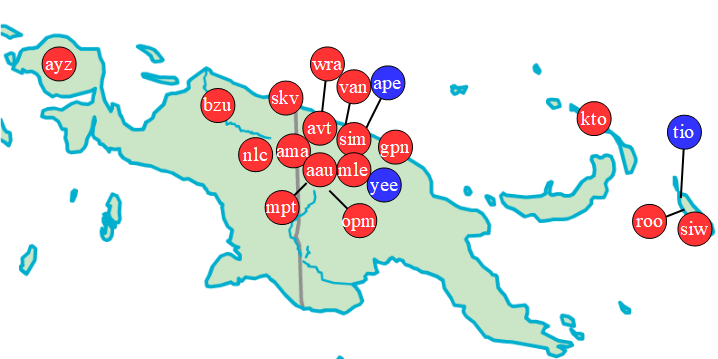
\includegraphics[width=\textwidth]{figures/09/Simple/fig6.png}
\caption{Occurrence of gender marking on nouns. Colors indicate: yes (blue), and no (red).}
\label{fig:Svard:6}
\end{figure}


Most languages of the sample (17 of 20) do not have overt gender marking, with Bukiyip, Teop, and Yimas being the only exceptions. In both Bukiyip and Yimas, gender is shown on nouns via suffixes; the Bukiyip noun suffixes are given in \tabref{tab:Svard:11}. Both languages are unusual in the sample by their having many noun classes (18 in Bukiyip, around a dozen in Yimas), many gender-indexing targets (both four or more), and semantic-formal assignment. In fact, these features are probably tightly interconnected with the overtness of gender. The combination of many genders and morphological gender assignment appears more common when noun classes are overtly distinct.


\begin{table}
\small
\begin{tabularx}{.9\textwidth}{lX>{\itshape}l>{\itshape}l>{\itshape}l>{\itshape}l}
\lsptoprule
Class &  Glossing & \multicolumn{2}{c}{\normalfont Example} & \multicolumn{2}{c}{\normalfont Noun suffix}\\
&  &\normalfont  singular &\normalfont  plural &\normalfont  singular &\normalfont  plural\\
\midrule
1 & betel nut & búb & búbús & {}-b/n & -bús\\
2 & village & wabél & walúb & {}-bél & -lúb\\
3 & feces & dewag & dewas & {}-g/-gú & -s/-as  \\
4 & woman & élmatok & élmagou & {}-k &  -ou/-eb\\
5 & banana & apam & apas & {}-m/-bal &  -s/-ipi/-bal\\
6 & moon & aun & aub & {}-n/-nú &  -b\\
7 & man & élman & élmom & {}-n/-nú & -m \\
8 & child & batawiny & batawich & {}-ny/-l & -ch/-has \\
9 & leaf & chuwup & chuwus & {}-p &  -s\\
10 & mosquito & aul & auguh & {}-l/-ny &  -guh\\
11 & dog & nobat & nobagw & {}-t/-tú &  \\
12 & sago leaves & lohuhw & lohulúh & {}-hw &  \\
13 & road & yah & yeh/yegwih & {}-{\normalfont V\textsubscript{1}}h & -{\normalfont V\textsubscript{2}}h  \\
14 & box & \multicolumn{2}{c}{\itshape kes} & {}-s &  -s\\
15 & small pig & \multicolumn{2}{c}{\itshape buligún} & {}-gún &  -gún\\
16 & garden & \multicolumn{2}{c}{\itshape yawihas} & {}-has &  -has\\
17 & personal names &  &  & {}- &  -\\
18 & place names &  &  & {}- &  -gún\\
\lspbottomrule
\end{tabularx}

\caption{Bukiyip noun classes and noun class suffixes (adapted from \citealt[10]{Conrad1991})}
\label{tab:Svard:11}
\end{table}


On the other hand, Teop (Austronesian, Oceanic) has a very different kind of marking. As mentioned above, Teop has a set of articles which obligatorily precede nouns, adjectives, and numerals. Thus, the latter two are indexation, while the articles preceding nouns are considered overt marking. The forms of the markers are shown in \tabref{tab:Svard:12}.


\begin{table}
\begin{tabular}{lllll}
\lsptoprule
& head (\textsc{sg}) & head \textsc{(pl)} & target \textsc{(sg)} & target \textsc{(pl)}\\
\midrule
Gender I-E & \itshape e & \itshape o & \itshape a & \itshape o\\
Gender I-A & \itshape a & \itshape o & \itshape a & \itshape o\\
Gender II & \itshape o & \itshape a & \itshape o & \itshape a\\
\lspbottomrule
\end{tabular}
\caption{Gender marking in Teop on articles preceding nouns (\citealt[322]{Mosel2000})}
\label{tab:Svard:12}
\end{table}


Note that Teop has two genders, one of which is divided into two subgenders. The reason for them not being separate gender is that the distinction is kept only on the articles preceding nouns, and never on the articles preceding adjectives and numerals. Thus, since overt gender marking cannot constitute gender as it is not indexation, Teop only has two genders.


This is very similar to the related Austronesian language Siar (not in the sample), which also has articles preceding nouns \citep{Frowein2011}. However, the Siar articles are not used in other contexts, so the absence of indexation renders Siar genderless. Nevertheless, a pronoun can be placed before e.g., an adjective, which is similar to the use of the Teop article. However, pronouns in Siar do not show any gender distinctions. The difference between Teop and Siar in this regard is shown in (\ref{ex:Svard:7}) and (\ref{ex:Svard:8}), respectively.


\ea
\label{ex:Svard:7}
Teop (Austronesian, Oceanic) (\citealt[326]{Mosel2000})\\
\gll \textbf{a} inu \textbf{a} rutaa\\
     \textsc{\textbf{art.i}} house \textsc{\textbf{art.i}} small\\
\glt `the small house / the house is small'
\z

\ea
\label{ex:Svard:8}
Siar (Austronesian, Oceanic) \citep[206]{Frowein2011}\\
\gll \textbf{Ép} rumai \textbf{i} mètèk.\\
     \textsc{\textbf{art.co1}} house \textsc{\textbf{3sg}} new\\
\glt `The house is new.'
\z


Finally, some languages have overt marking in some cases or at least something resembling it. One example is Kuot (isolate), where some nouns belong to various declension classes (as defined by noun endings), which in turn belong to a certain gender (\citealt[176]{Lindstroem2002}). Another example is Rotokas (North Bougainville), which has noun suffixes expressing both number and gender \citep[41]{Robinson2011}. However, these are not always present: in (\ref{ex:Svard:9}a), \textit{aveke} `stone' has a feminine singular suffix, but in (\ref{ex:Svard:9}b) it remains unmarked.

\protectedex{%
\ea
\label{ex:Svard:9}
Rotokas \citep[42]{Robinson2011}\\
\begin{xlist}
\ex
\gll riako-va \textbf{aveke-va} peka-e-vo uva rakoru keke-e-vo uva kea-o-e oisio uo-va\\
woman-\textsc{sg.f} \textbf{stone-}\textsc{\textbf{sg.f}} turn.over-3\textsc{sg.f-ipst} and snake look.at-\textsc{3sg.f-ipst} and\textsc{} mistake.for-\textsc{3sg.f-ipst} as\textsc{} eel\textsc{{}-sg.f}\\
\glt `The woman turned over to the stone and saw a snake but mistook it for an eel.'

\ex
\gll kaveakapie-vira \textbf{aveke} tovo-i-vo uva kove-o-e\\
insecure-\textsc{adv} \textbf{stone} place-\textsc{3pl-ipst} and fall-3\textsc{sg.f-ipst}\\
\glt `They placed the stone insecurely and it fell down.'
\end{xlist}
\z
}%

Since gender marking on nouns is not always present, Rotokas cannot be said to have obligatory overt marking.

\section{ Typological comparison}
\label{sec:Svard:4}

This section compares the results of this study with previous research on Africa and the world as a whole. The data on Africa is from \citet{DiGarbo2014}, which used the same five criteria of this study to investigate a variety sample of 100 languages. The data on the world as a whole is based on the three \textit{WALS} chapters on gender by  \citet{Corbett2013,Corbett2013a,Corbett2013b}. These three \textit{WALS} chapters correspond to the first three classification criteria of this study. Unfortunately, the remaining two have no corresponding \textit{WALS} data, rendering the final two criteria comparable only for New Guinea and Africa.



Some care had to be taken when comparing the results, since the samples are of different types. Whereas this study employs a variety sample, Corbett uses a proportional sample (of 257 languages) (see \sectref{sec:Svard:2}). Di Garbo also uses a variety sample (of 100 languages) although with some differences, most importantly the inclusion of 16 non-gendered languages as well as being intentionally genealogically skewed. To make the data comparable, languages without gender have been omitted from Corbett's and Di Garbo's samples in this section, leaving 112 languages for Corbett and 84 for Di Garbo.



\textit{Classification criterion 1: Sex-based and non-sex-based gender systems (\sectref{sec:Svard:3.1}).} In the sample of this study, sex-based systems are by far more common, with only Teop (Austronesian, Oceanic) having a non sex-based system. In comparison, in Di Garbo's (\citealt*[63]{DiGarbo2014}) sample, 48 languages (57\%) had sex-based gender systems and 36 languages (43\%) non-sex-based gender systems. In Corbett's (2013b) sample, 84 languages (75\%) have sex-based systems and 28 (25\%) non-sex-based. A comparison of the percentage distributions is shown in \figref{fig:Svard:7}.


\begin{figure}
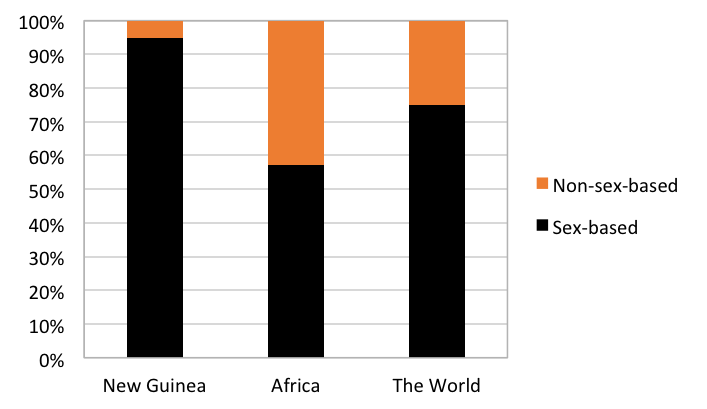
\includegraphics[width=\textwidth]{figures/09/fig7.png}
\caption{Sex-based and non-sex-based systems in New Guinea, Africa and the world}
\label{fig:Svard:7}
\end{figure}


Sex-based systems are more common in all samples, although even more so in the sample from New Guinea. According to Corbett's (\citealt*{Corbett2013a}) data, non-sex-gender systems are actually uncommon in most regions, being found primarily in the Niger-Congo languages of Africa, which account for the vast majority of non-sex-based systems in the sample. More specifically for Africa, in most cases only one system occurs in an entire family: this is true e.g., for the Bantu, Mel, and North-Central Atlantic families, which together account for 33 of the 36 non-sex-based gender systems in Di Garbo's sample. It is therefore not surprising that the non-sex-gender systems are relatively common, since 31\% of the gendered languages (26/84) in Di Garbo's sample are Bantu languages.



An interesting discussion about the differences between sex-based and non-sex-based systems is presented by \citet{Luraghi2011}, who argues that they have different diachronic origins, with non-sex-based systems originating from the grammaticalization of classifiers and sex-based systems from agreement from different morphosyntactic behaviors of groups of nouns. Since sex-based systems are more common, it is thus not surprising that they are the primary ones in New Guinea. It is likely not a coincidence that the only non-sex-based gender system of the sample is found in an Austronesian language, a family remarkably devoid of gender but abounding with classifiers.


\textit{Classification criterion 2: Number of genders (\sectref{sec:Svard:3.2})}. In the sample of this study, eleven languages (55\%) have only two genders, three languages (15\%) three genders, one language (Mian; TNG, Ok-Oksapmin) (5\%) four genders, and the final five languages (25\%) five genders or more. In Di Garbo's (\citealt*[65]{DiGarbo2014}) sample, 42 languages (50\%) have only two genders, seven languages (8\%) three genders, one (Ju{\textbar}'hoan; Kxa) (1\%) four genders, and the final 34 languages (40\%) five genders or more. In Corbett's (\citealt*{Corbett2013}) sample, 50 languages (45\%) have only two genders, 26 languages (23\%) three genders, 12 languages (11\%) four genders, and the final 24 (21\%) five genders or more. A comparison between the percentage distributions is shown in \figref{fig:Svard:8}.


\begin{figure}
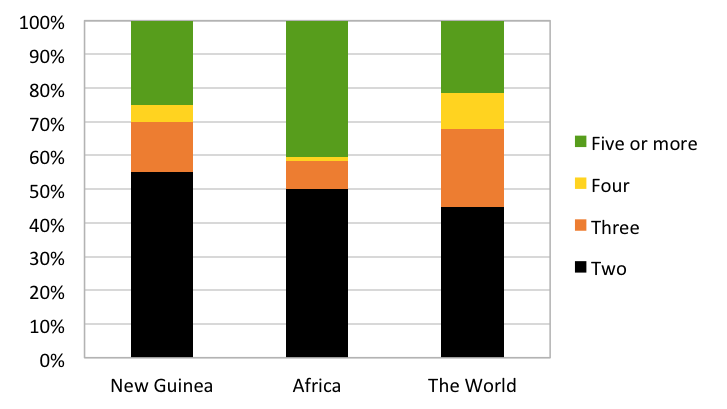
\includegraphics[width=\textwidth]{figures/09/fig8.png}
\caption{Number of genders in New Guinea, Africa and the world}
\label{fig:Svard:8}
\end{figure}

The distributions in all three samples are similar to a large extent, with two-gender systems being present in around half of the languages. In Africa, large systems are much more common than in New Guinea or the world as a whole. However, this may once again be because of the sample. As mentioned before, 31\% of the languages present in Di Garbo's (\citealt*{DiGarbo2014}) sample are Bantu languages, all of which have very large gender systems. In the sample of this study, however, the rather large Torricelli and Lower Sepik-Ramu families, which according to \citet[372]{Foley2000} have large systems, are represented only by Bukiyip and Yimas respectively (i.e., 10\% of the sample). It is thus very probable that the similarities between the distribution numbers of genders in New Guinea and Africa actually are greater than indicated here.


\textit{Classification criterion 3: Gender assignment (\sectref{sec:Svard:3.3}).} This criterion is less straightforward to compare, since this study uses three values (transparent semantic, semantic and formal, and opaque), whereas \citet{DiGarbo2014} and \citet{Corbett2013b} use only two (semantic, and semantic and formal). For the purpose of this comparison, the languages of the purely semantic and semantic + opaque groups are added somewhat tentatively into a semantic group. While this may appear misleading, it is important to note that the researchers investigating these languages considered them as having semantic gender assignment and no traces of formal assignment rules have been identified by the present author. Indeed, both languages exemplified in \citet{Corbett2013b}, Bininj Gun-Wok (Gunwinygic; northern Australia) and Russian, would be considered opaque using the values of this study.



In the sample of this study, 16 languages (80\%) exhibit semantic gender assignment, whereas only four languages (20\%) show semantic and formal assignment.  In comparison, in Di Garbo's (\citealt*[67]{DiGarbo2014}) sample, six languages (7\%) have semantic assignment, 76 languages (90\%) semantic and formal assignment, while the remaining two languages (2\%) have unknown assignment (disregarded in \figref{fig:Svard:9}). In Corbett's (\citealt*{Corbett2013b}) sample, 53 languages (47\%) exhibit semantic assignment, and 59 languages (53\%) semantic and formal assignment. A comparison between the percentage distributions is shown in \figref{fig:Svard:9}.


\begin{figure}
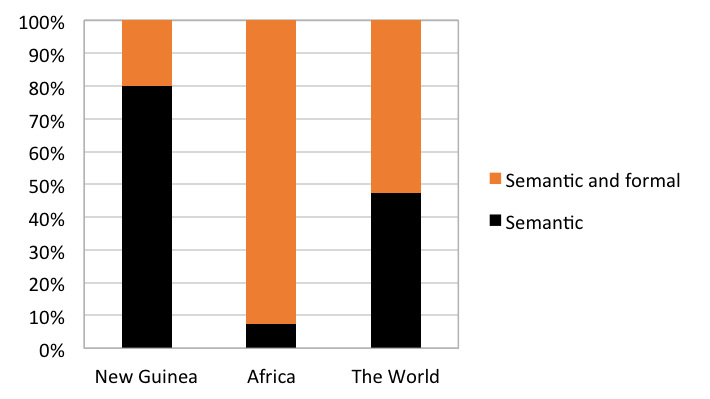
\includegraphics[width=\textwidth]{figures/09/fig9.png}
\caption{Gender assignment in New Guinea, Africa and the world}
\label{fig:Svard:9}
\end{figure}


As can be clearly seen in \figref{fig:Svard:9}, in New Guinea, semantic assignment is by far more common, while it is by far the most uncommon form of gender assignment in Africa, including of course the Bantu languages. In the world as a whole, the ratio is more or less equal. Thus, New Guinea and Africa both represent two extremes while the world as a whole is more average. However, according to \citet{Corbett2013b}, semantic and formal assignment is mostly found in the Indo-European, Afro-Asiatic, and Niger-Congo families, which together represent a large amount of the languages of the world.



It is not surprising that semantic and formal assignment appears more often in Di Garbo's and Corbett's samples than in New Guinea, since no family is represented with more than three members in this study. Bukiyip (Torricelli, Arapesh) and Yimas (Lower Sepik-Ramu, Lower Sepik) both belong to rather large families, so it is possible that a proportional sample would show that semantic and formal assignment indeed is more common than it appears here. Nevertheless, it is interesting that it occurs in few families, both in New Guinea and the world, which \citet{Corbett2013b} relates to these systems necessarily being older. As argued by \citet{Luraghi2011}, this implies that most gender systems of Africa are old. Exclusive semantic assignment is however found in both older and younger systems, and thus it cannot be claimed that the predominance of semantic assignment indicates that those systems are young. Interestingly, semantic and formal assignment is found in Nalca (TNG, Mek), which has a very young gender system (\citealt{Waelchli2018}).



\textit{Classification criterion 4: Number of gender-indexing targets (\sectref{sec:Svard:3.4}).} In the sample of this study, four languages (20\%) have only one gender-indexing target, another four languages (20) two targets, two languages (10\%) three targets, and the final ten languages (50\%) four or more targets. In Di Garbo's (\citealt*[68]{DiGarbo2014}) sample, five languages (6\%) have only one gender-indexing target, 16 languages (19\%) two targets, 28 languages (33\%) three targets, and finally 33 languages (39\%) four targets or more. No data was available for the remaining two languages. A comparison of the percentual distributions is shown in \figref{fig:Svard:10}.


\begin{figure}
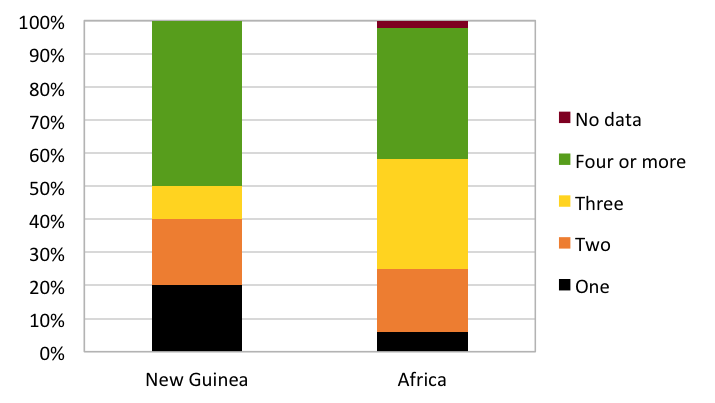
\includegraphics[width=\textwidth]{figures/09/fig10.png}
\caption{Number of gender-indexing targets in New Guinea vs.\ Africa}
\label{fig:Svard:10}
\end{figure}

Four or more gender-indexing targets is the most common number in both samples, accounting for slightly less than half of all languages. Furthermore, systems of only two targets account for around a fifth of the languages in both samples. As for the two remaining values, the relationships are the opposite: systems of three targets are common in Africa but rare in New Guinea, whereas one-target systems occur in a fifth of the New Guinean languages but only 6\% of the African languages. However, once again it is probable that these differences are largely due to larger families with more mature gender systems being better represented in Di Garbo's (\citealt*{DiGarbo2014}) sample, while languages from smaller families with possibly less mature gender systems constitute a large part of the sample of this study.


\textit{Classification criterion 5: Occurrence of gender marking on nouns (\sectref{sec:Svard:3.5}).} In the sample of this study, three languages (15\%) have overt gender marking, whereas the remaining 17 (85\%) do not. In Di Garbo's sample 69 languages (82\%) have overt gender marking and 15 (18\%) do not. A comparison between the percentage distributions is shown in \figref{fig:Svard:11}.


\begin{figure}
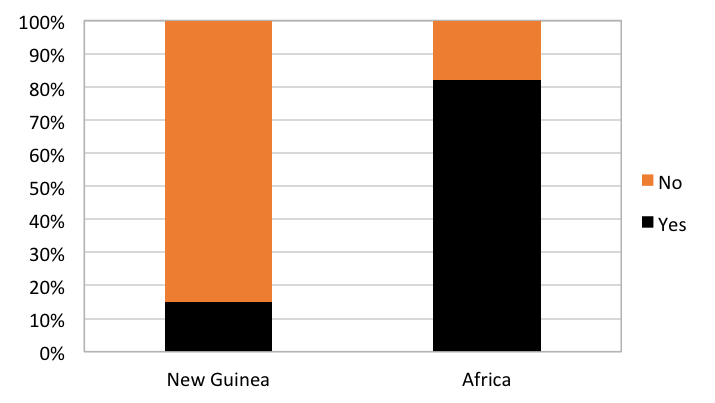
\includegraphics[width=\textwidth]{figures/09/fig11.png}
\caption{Occurrence of gender marking on nouns in New Guinea vs.\ the world}
\label{fig:Svard:11}
\end{figure}

As the figure shows, there is a major disparity between the presence of gender marking on nouns in New Guinea and Africa. In New Guinea, overt gender marking is rare and occurs in only three languages in the sample, whereas in Africa it occurs in the vast majority of languages.

There is an interesting correlation between this distribution and the one of gender-assignment shown in \figref{fig:Svard:4}. Thus, semantic assignment without gender marking on nouns is the norm in New Guinea, whereas semantic and formal assignment with gender marking on nouns is the norm in Africa. This correlation is hardly coincidental. A gender system with assignment based on formal criteria benefits greatly from overt gender; in an exclusively semantic system however, obligatory overt gender has no function in gender assignment.

To summarize, it can be confidently stated that the gender systems of New Guinea and Africa are very different. Much of this depends on the hegemony of Bantu languages in Africa (as represented by Di Garbo's sample), which makes the distribution of values much less diverse than in the sample of this study. Nevertheless, the most important differences are (1) the prevalence of semantic and formal assignment and overt gender in Africa, while the exact opposite is true in New Guinea, and (2) as the observation that non-sex-based genders are much more common in Africa. This clearly shows that the two regions have gender systems of very different types. Reasons for this definitely include sample size and technique, but it also suggests that the gender systems of New Guinea may have different diachronic origins.

As for New Guinea in relation to the world as a whole, the above data and figures show that the distribution of values of the three classification criteria is rather similar in New Guinea and the world. In fact, most of the smaller differences can probably be accounted for by sample size. Nevertheless, the main conclusion is that the languages of New Guinea seem to be remarkably representative of the languages of the world, but another study with a proportional sample from New Guinea would elucidate this further.

\section{Special characteristics}

In this section, four characteristics of the gender systems of New Guinea are highlighted, two of which reflect characteristics mentioned by \citet{Foley2000}, viz., gender assignment based on size and shape, and the occurrence of two separate gender systems. The other two, viz., no gender distinctions in pronouns and gender marking on verbs, pertain to two typologically uncommon characteristics.  Although these do not occur in all languages of the sample, they are found in geographically and genealogically distant languages and are all characteristic of the region.

\subsection{ Size and shape}
\label{sec:Svard:5.1}
Four languages in the sample (20\%) share the property of having size and shape as important criteria for gender assignment. While gender assignment in many languages may carry some form of size- or shape-based rules, the rules discussed here all share the feature that nouns denoting tall, long, or thin objects are considered masculine, whereas nouns denoting short, thick, or round objects are feminine. In addition, they are all core assignment criteria. The languages in the sample exhibiting this feature are: Abau (Sepik), Manambu (Ndu), Skou (Sko), and Taiap (isolate). Their rules based on shape and size are shown in \tabref{tab:Svard:13}.


\begin{table}
\begin{tabularx}{\textwidth}{lQQ}
\lsptoprule
 Language &  Masculine\footnotemark{} & Feminine\\\midrule
Abau & {{}- large}

{{}- three-dimensional}

{}- long and extended & {{}- small}

{{}- two-dimensional (i.e., very thin)}

{}- round with little height\\
Manambu & {{}- large}

{}- long & {{}- small}

{}- round\\
Skou & {{}- large}

{}- long, thin & {{}- small}

{}- round, squat\\
Taiap & {{}- large}

{}- long, high, thin & {{}- small}

{}- round, stocky\\
\lspbottomrule
\end{tabularx}

\caption{Gender assignment rules based on size and shape in the sample}
\label{tab:Svard:13}
\end{table}

\footnotetext{`Non-feminine' in Skou.}

In these four languages, size and shape are important criteria for gender assignment. One example mentioned in \sectref{sec:Svard:3.1} above is Abau, which has two genders: masculine and feminine. Humans, along with spirits and domesticated animals, are assigned gender based on their sex, whereas abstract entities are feminine \citep[47]{Lock2011}. However, animals and concrete inanimate objects are assigned their gender based on shape and size. Large, three-dimensional, and/or long and extended objects are masculine, while small, two-dimensional (i.e., very thin), and/or round objects with little height are feminine \citep[47]{Lock2011}. Thus, \textit{su} `coconut' (three-dimensional), \textit{now} `tree' (long), and \textit{hu} `water' (liquid) are masculine, while \textit{iha} `hand' (flat) and \textit{hne} `bird's nest' (round with little height) are feminine (\citealt[48--50]{Lock2011}).



It is important to distinguish systems such as the ones above from diminutives. In some languages, diminutives constitute separate genders, such as in Motuna (South Bougainville) (\citealt[68--69]{Onishi1994}). However, the four languages above show the peculiar characteristics that (1) size and shape function as assignment criteria for the masculine and feminine genders, and (2) they constitute opposing criteria, and (3) they show the same pattern of large/long vs.\ small/round.


In the sample, size and shape constitute important gender assignment criteria in only these four languages, but similar systems are present in other languages. Rotokas exhibits some similarities with these gender assignment rules in two ways. Firstly, one class of nouns belonging to the masculine gender consists of inanimate objects associated with male culture, but also includes long or thin objects. However, no comparable feminine gender assignment rule has been found. Furthermore, this is appears to be only a peripheral gender assignment rule. Secondly, Rotokas has a set of classifiers based on shape and size, classifying nouns based on their being round, narrow, or long. While this is not related to any masculine-feminine opposition, it nonetheless bears some resemblance to these systems.


Another interesting example is Mian (TNG, Ok). Mian has four genders, viz., male, female, neuter 1, and neuter 2, none of which has gender assignment rules resembling those of size and shape (\citealt[171--176]{Fedden2011}). However, around 50 verbs require the use of a classificatory prefix, which has two functions: firstly, it encodes the direct object of transitive verbs and the subject of intransitive verbs, and secondly it classifies it according to characteristics of the referent, viz., sex, shape, and function \citep[185]{Fedden2011}. This classification system, which is separate from the gender system, includes classes for e.g., long or flat objects, and in some cases overlaps with the gender system (e.g., some neuter 1 nouns are included in the masculine class. A table illustrating the overlap between the two systems is shown in \tabref{tab:Svard:NEW}.

%\begin{figure}
%
%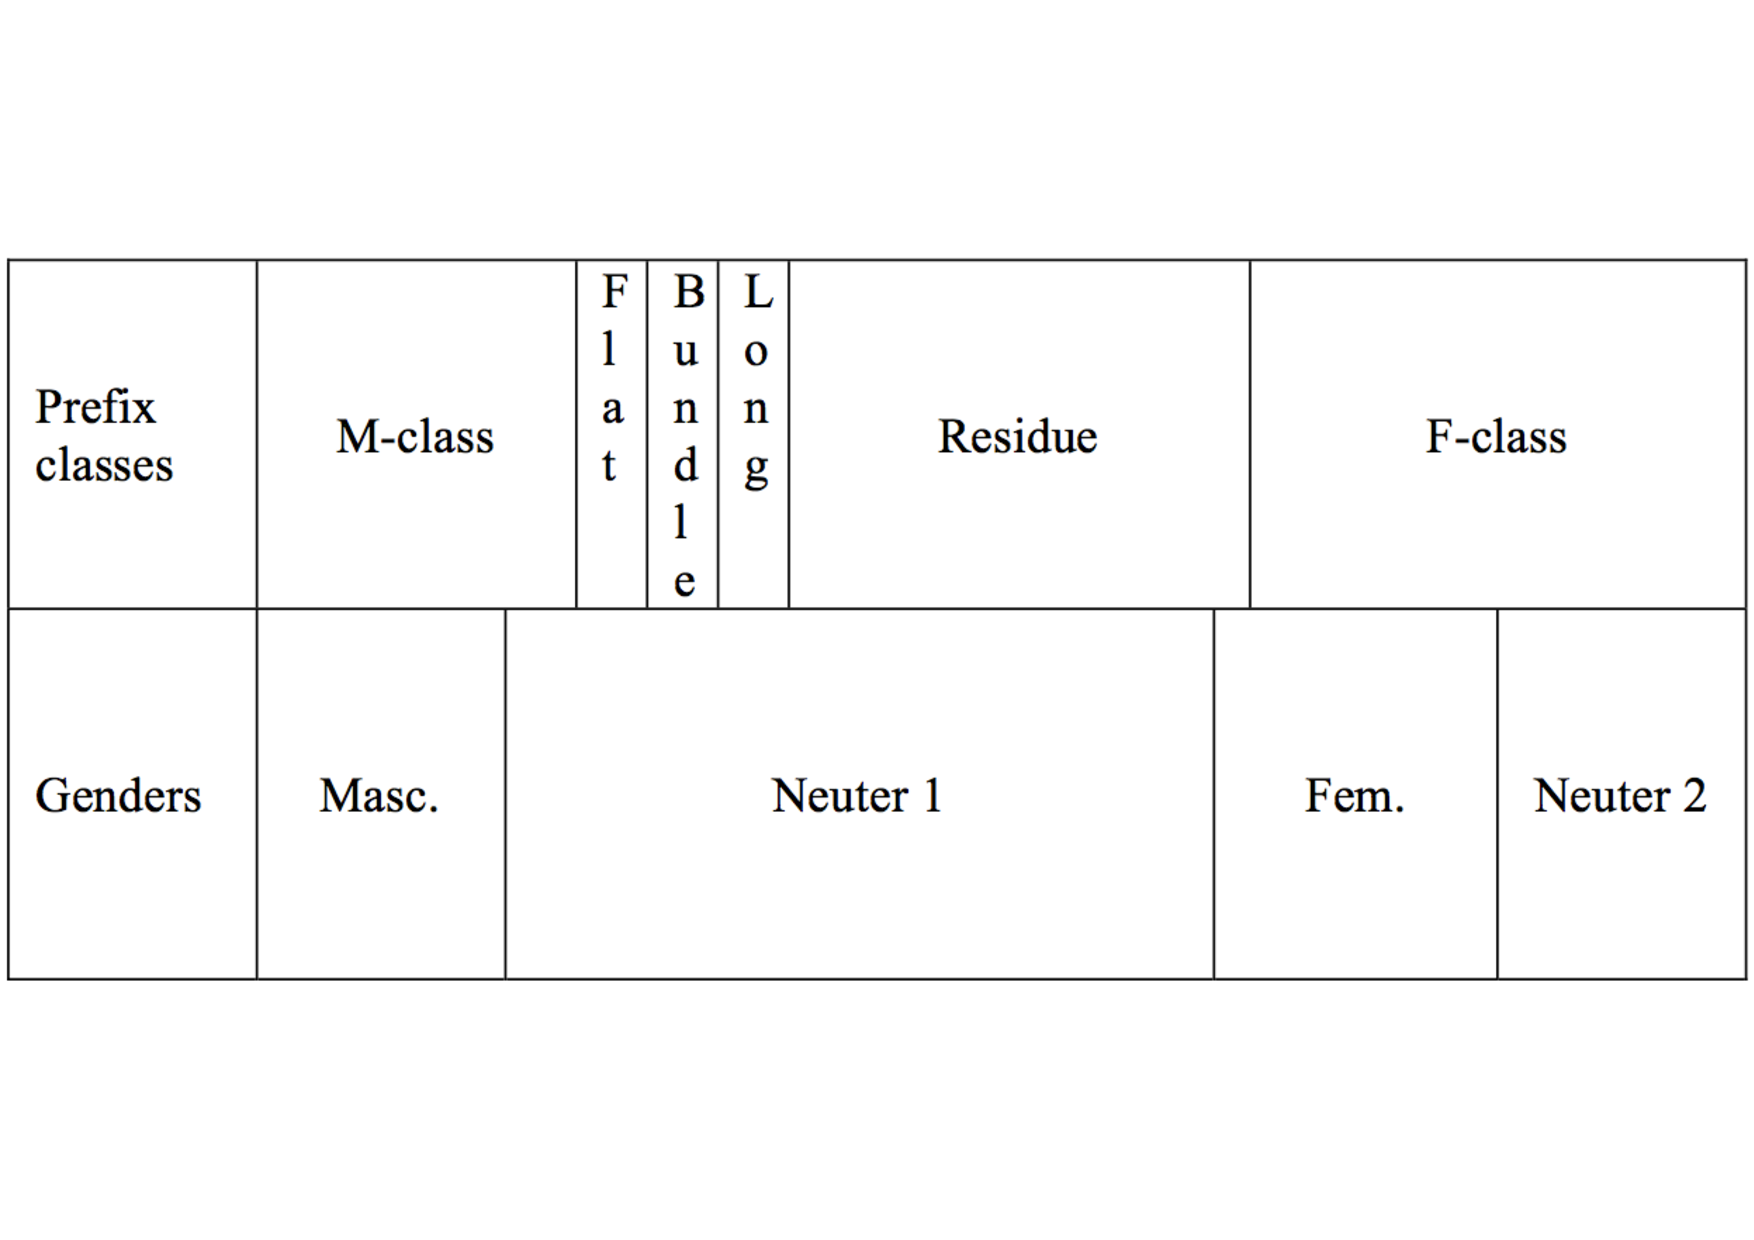
\includegraphics[width=.8\textwidth]{figures/09/Fedden.pdf}
%
%\caption{Overlap between the gender and verb prefix classes of Mian (from %\citealt[188]{Fedden2011}).
%%The term ``covering'' is employed rather than ``flat'' since the latter is only mentioned in the figure while the former is employed throughout the text.
%}
%\label{fig:Svard:12}
%\end{figure}

\begin{table}[htb]
\small
\begin{tabularx}{\textwidth}{lQQQQ}
\lsptoprule
  & Masculine & Feminine & Neuter 1 & Neuter 2 \\
\midrule
M-classifier & man, boy, boar & -- & sleeping bag, plate, mosquito net & -- \\
F-classifier & -- & woman, girl, sow & -- & house, steel axe, money \\
Long & -- & -- & tobacco, eating implement, bush knife & -- \\
Bundle & -- & -- & string bag, plastic bag & -- \\
Covering & -- & -- & blanket, band aid & -- \\
Residue & -- & tortoise, scorpion & cassowary egg, plane, hat & -- \\
\lspbottomrule
\end{tabularx}
\caption{Overlap between the gender and verb prefix classes of Mian (adapted from \citealt[34]{Fedden2017}). Cells with examples show the attested combinations.}
\label{tab:Svard:NEW}
\end{table}


Assigning genders based on shape and size is not very common in the languages of the world (\citealt[chap.~11]{Aikhenvald2000}). Outside of New Guinea, it occurs e.g., in some Afroasiatic languages, such as Oromo and Amharic, Central Khoisan, and Cantabrian Spanish (\citealt[277]{Aikhenvald2000}; \citealt[191]{Heine1982}). However, size as an assignment criterion is widespread in Africa, where it e.g., occurs in diminutive and augmentative genders as reported by \citet{DiGarbo2014}. An example is in Tonga, where `boy' (noun class 1) can shift to the diminutive noun class 12 to highlight smallness:


\ea
Tonga (Bantu) (\citealt[147]{DiGarbo2014}; from \citealt[21]{Carter2002})\\
\begin{xlist}
\ex
\gll mu-sankwa\\
     \textsc{cl1-}boy\\
\glt `boy'
\ex
\gll tu-sankwa\\
     \textsc{cl12-}boy\\
\glt `small boy'
\end{xlist}
\z


As for New Guinea, its prevalence specifically in the Sepik area has led \citet[113]{Aikhenvald2008} to suggest that gender assignment based on size and shape may actually be an areal feature of the Sepik area. Indeed, all four languages in this sample found to have such systems are spoken in or near the Sepik area: Abau (Sepik) and Manambu (Ndu) are spoken inside it, while Skou (Sko) and Taiap (isolate) are spoken in relatively adjacent areas. Another oft-cited example is Alamblak (\citealt{Bruce1984}; not in the sample), also a Sepik language of the same area, which has a system similar to that of Manambu \citep[112]{Aikhenvald2008}.



Thus, gender assignment according to size and shape appears to be an areal feature, since it occurs in a wide area and in languages of different families. This gives rise to an important question. Why would a system of gender assignment be areal when gender is such a stable and not easily borrowed feature?  Although this is far beyond the scope of this study, there are some hints that this may be part of a larger cultural classificatory system (i.e., perceptual, not linguistic). The reason for such a possibility is that besides occurring in and around the Sepik area, there are other New Guinean languages where nouns are grouped based on size and shape with other nouns denoting male or female referents, even when there is no gender system. This is most apparent in the TNG languages of the central highlands; nouns in these languages can be categorized by the type of stance verb they occur with, so that males or large, long, or tall objects occur with `stand', whereas women or small, short, or round objects occur with `sit'  \citep[372]{Foley2000}. An example of such a language is Enga (Engan; New Guinea Highlands; not in the sample), which has seven different stance verbs, including \textit{katengé} `stand', which is used for referents considered tall, large, strong, and/or powerful such as `men', `house', and `tree', and \textit{pentengé} `sit', which is used for referents considered small, squat, horizontal, and/or weak such as `woman', `possum', and `pond' (\citealt[158--159]{Aikhenvald2000}; \citealt{Rumsey2002}). Thus, it appears that the perception of large, long, or tall objects being related to males and/or masculinity, and small, short, or round objects being related to females and/or femininity is a characteristic of New Guinea that extends beyond gender systems or the Sepik area.


\subsection{ Two separate systems of noun classification}
\label{sec:Svard:5.2}

In most gendered languages, gender constitutes a single system where each noun is assigned to a single class which is reflected in the form of indexation targets. However, there are also languages with two separate systems, both of which appear to constitute or be related to gender systems, but which occur with different types of targets. Thus, in such a language each noun is assigned to not just one class, but to two different classes. In the sample of this study, five languages have such systems (see \tabref{tab:Svard:14}).

%%please move \begin{table} just above \begin{tabular
\begin{table}
\begin{tabularx}{\textwidth}{XXXX}
\lsptoprule
Separate systems & No. of lgs. & \% & Language\\
\midrule
Yes & 5 & 25\% & {Abau}

{Burmeso}

{Mian}

{Motuna}

Rotokas\\
No & 15 & 75\% & {Ama}

{Au}

{Bukiyip}

{Kuot}

{Manambu}

{Maybrat}

{Mende}

{Nalca}

{Oksapmin}

{Skou}

{Taiap}

{Teop}

{Walman}

{Warapu}

Yimas\\
\midrule
Total: & 20 & 100\% & \\
\lspbottomrule
\end{tabularx}
\caption{Languages in the sample with separate gender and noun class systems}
\label{tab:Svard:14}
\end{table}



Even in the small sample of this study, the two separate systems range from languages with two more or less equally complex systems (i.e., with similar numbers of forms and uses) to languages where one system is more complex whereas the other is much less so. In order to retain the typological comparability of the results, a distinction has been made between systems of gender and systems of noun classifiers. However, it should be stated that there is a thin line between the two and they most certainly constitute two edges of the same continuum. Following these, four of the five languages with two systems of noun classification can be argued to exhibit one gender system and system of noun classifiers, whereas only Burmeso has two systems which both satisfy the conditions for gender systems. In the first system, Burmeso has three genders (masculine, feminine, and neuter), appearing as adjectival agreement suffixes (\ref{ex:Svard:11}a), which are further divided into two subgenders (animate and inanimate), each depending on the plural agreement marker (\citealt[105--106]{Donohue2001}). However, in the second system (which Donohue calls a noun class system), Burmeso has six genders (I--VI), which occur in verbal agreement prefixes (\ref{ex:Svard:11}b) \citep[101]{Donohue2001}. In addition, there are three words which take both kinds of agreement: \textit{{}-aysa-} `one', \textit{{}-akasu-} `all', and \textit{{}-asna-} `white' (\ref{ex:Svard:11}c).


\ea
\label{ex:Svard:11}
Burmeso (isolate) (\citealt[105, 109, 100]{Donohue2001})\\
\begin{xlist}
\ex
\gll Da de koya bek-\textbf{abo}.\\
     \textsc{1sg} \textsc{1sg.poss} grandfather good-\textsc{\textbf{m.sg}}\\
\glt `My grandfather is well.'
\ex
\gll Da mibo \textbf{j}{}-ihi-maru.\\
     \textsc{1sg} banana \textsc{\textbf{v.sg}}{}-see-\textsc{tpst}\\
\glt `I saw a banana.'
\ex
\gll Sunam \textbf{n}{}-asna-\textbf{b}.\\
     axe.\textsc{sg} \textsc{\textbf{iii.sg}}\textsc{{}-}white\textsc{{}-}\textsc{\textbf{m.sg}}\\
\glt `(The) axe is white.'
\end{xlist}
\z


As expected from the number of genders being different, the two systems use different assignment rules. Both systems are sex-based with importance clearly put on sex and animacy, but none of them have only transparent semantic rules: e.g., `wind' is neuter/III, `rain' masculine/IV, and `star' masculine/III) (\citealt[103--107]{Donohue2001}). A comparison of the overlap of the two systems is exemplified in \tabref{tab:Svard:15}, showing how members are assigned to both systems.

\begin{landscape}
\thispagestyle{empty}

%%please move \begin{table} just above \begin{tabular
\begin{table}
\small
\begin{tabularx}{\textwidth}{lQQQQQQ}
\lsptoprule

Class & Masculine & Feminine & Neuter & {M}

inanimate & {F}

inanimate & {N}

animate\\
\midrule
I & {male humans}

{(most birds, animals etc.)}

\textsc{2sg pro} & {(birds of paradise)}

{pigeons}

sago garden & sea & neck & – & {sea}

wound\\
II & \textsc{1sg pro} & female humans & {nose}

{ear}

eye & – & small goanna & {string}

{shapes}

{sago rinser}

(lower)\\
III & {axe}

{papaya}

ground bird & – & {(some small animals)}

bench & {papaya}

{rattan}

{mountain}

{lake}

{(all tubers)}

{upper sago}

{trough}

female child & goanna & –\\
IV & head, flesh, feces, finger, elbow, sun, cloud, rain, sand, mud & – & – & – & – & –\\
V & – & – & (arrows) & banana & – & –\\
VI & – & – & – & coconut & – & –\\
\lspbottomrule
\end{tabularx}
\caption{Comparison between genders and noun classes in Burmeso (adapted from \citealt[108]{Donohue2001}). As in the source, the subgenders of the masculine, feminine, and neuter genders are shown.}
\label{tab:Svard:15}
\end{table}

\end{landscape}


Near the other end of the spectrum lies Rotokas (North Bougainville). Rotokas has three genders, viz., masculine, feminine, and neuter, which appear e.g., in pronouns, demonstratives, adjectives, and verbs (\ref{ex:Svard:12}a) \citep{Robinson2011}. However, Rotokas also has noun classifiers, which consist of two different sets. The first set consists of four classifiers; these distinguish between shape and size, and importantly occur on both attributive (\ref{ex:Svard:12}b) and predicative modifiers of the classified noun \citep[50]{Robinson2011}.


\ea
\label{ex:Svard:12}
Rotokas (North Bougainville) (\citealt[149, 50]{Robinson2011})\\
\begin{xlist}
\ex
\gll Pita vaio ora Kariri ava-\textbf{si}{}-ei voka-sia\\
     P. \textsc{dl.anim} and K. go-\textsc{\textbf{3dl.m}}\textsc{{}-prs} walk-\textsc{dep.seq}\\
\glt `Peter and Kariri are going for a walk.'
\ex
\gll gorupasi \textbf{isi} rutu karuvera \textbf{isi} aio-a-voi\\
     strong \textsc{\textbf{cl.}}\textbf{round} very Singapore \textsc{\textbf{cl}}\textbf{.round} eat-\textsc{1sg-prs}\\
\glt `I am eating a really strong Singapore fruit.'
\end{xlist}
\z


The other set of classifiers, which has more members and have collective meanings, occurs following, or instead of, the classified noun \citep[51]{Robinson2011}. Interesting to note is that classified nouns become neuter in regards to gender agreement \citep[53]{Robinson2011}.


Abau also exhibits a clear noun classifier system (Table \ref{tab:Svard:16}). There are two genders in Abau, masculine and feminine, which follow opaque gender assignment rules and appear in e.g., pronouns and demonstratives. However, the numerals `one', `two', and `three' do not agree with this system, but instead take one of twelve prefixes based on semantic criteria of the referent. However, the same noun can be used with different numeral classifiers in order to indicate a specific referent, so that e.g., \textit{su piron} `one coconut' refers to the whole coconut palm and not just the fruit, since class 5 signals long objects, while \textit{su kamon} `one coconut' is used when referring to just the fruit, since class 2 does not carry the semantic feature of length. It is thus evident that this system of noun classifiers is not lexically determined by the noun itself and thus not a gender system.

%%please move \begin{table} just above \begin{tabular
\begin{table}
\begin{tabularx}{\textwidth}{lX>{\itshape}l>{\itshape}l>{\itshape}l}
\lsptoprule

Class & Characteristics & \normalfont One & \normalfont Two & \normalfont Three\\
\midrule
1 & Human beings; spirits & pru-eyn & pru-eys & pru-ompri\\
2 & Non-human & ka-mon & k-reys & k-rompri\\
3 & Small objects with some volume & na-mon & na-reys & na-rompri\\
4 & Flat surface objects; experience nouns & si-rom & s-eys & s-ompri\\
5 & Long, relatively thin objects & pi-ron & pi-reys & pi-rompri\\
6 & Geographical locations & u-mon & u-reys & u-rompri\\
7 & Flat objects with hardly any volume & i-mon & i-reys & i-rompri\\
8 & Certain type trees & li-mon & li-reys & li-rompri\\
9 & Bundles of long non-cut items & ein-mon & ein-deys & ein-rompri\\
10 & Temporal & leik-mon & leik-reys & leik-rompri\\
11 & Bundles of long cut items & hnaw-mon & hnaw-reys & hnaw-rompri\\
12 & Part of a long object & houk-mon & houk-reys & houk-rompri\\
\lspbottomrule
\end{tabularx}
\caption{Numeral classifiers in Abau (adapted from \citealt{Lock2011}:57)}
\label{tab:Svard:16}
\end{table}



Mian has a similar albeit different system. In Mian, there is a set of verbal classificatory prefixes which are divided into six classes (\tabref{tab:Svard:17}). These prefixes are used only for around 50 verbs, the vast majority of which refer to forms of object manipulation, movement, and handling \citep[172]{Fedden2011}. Once again, this is clearly not a full-fledged gender system, but rather a classifier system.


\begin{table}
\begin{tabularx}{.8\textwidth}{lX>{\itshape}p{2cm}>{\itshape}p{2cm}}
\lsptoprule
Class & Characteristics & \multicolumn{2}{c}{Verbal classificatory prefixes}\\
&  & \normalfont Singular & \normalfont Plural\\
\midrule
1 & Masculine & do(b)- & \multirow{2}{*}{do(l)-, dl-}\\
2 & Feminine & om- & \\
3 & Long object & to(b)- & tebe(l)-\\
4 & Bundle-like object & go(l)- & gule(l)-\\
5 & Flat object & gam- & geme(l)-\\
6 & Residue class & o(b)- & o(l)-\\
\lspbottomrule
\end{tabularx}

\caption{Classifiers in Mian (adapted from \citealt[172]{Fedden2011})}
\label{tab:Svard:17}
\end{table}


Finally, Motuna is a particularly interesting case since its secondary system lies near the boundary between genders and noun classifiers. Besides its gender system (described in \sectref{sec:Svard:3.3}), Motuna has another noun classification system consisting of 51 different classifiers, which are visible in the forms of adjectives, verbs, participial clauses, articles, demonstratives, possessive pronouns, and numerals (\citealt[162--163]{Onishi1994}). Thus, as for indexation, the system is very reminiscent of a gender system. However, the classes are not lexically determined, meaning that the same noun may occur with various classifiers depending on the referent. Furthermore, as expected for a noun classifier system, the classifiers refer properties such as size, shape, type of vegetable, and collectives (e.g., `bundle', `packet'). Thus, \textit{moo} `coconut' can occur with classes 4 \textit{{}-mung} `plant/fruit/nut/egg/things made of plant/coin' (> `coconut (nut/tree)), 5 \textit{{}-ri} `nut with hard shell' (> `coconut'), 6 \textit{{}-mo'} `bunch of nuts' (> `coconut'), 13 \textit{{}-ri'} `round object' (> `coconut'), and 30 \textit{{}-ita} `half/side' (> `half coconut shell') (\citealt[166--167]{Onishi1994}). Therefore, this system in Motuna is a system of noun classifiers, not genders.



Despite the small size of the sample used in this study, the proportion and the geographic and genealogical spread of languages with two separate systems of nominal classification indicate that the phenomenon is rather common and widespread in New Guinea. Besides the languages of this study, two of which are mentioned by \citet[373]{Foley2000}, viz., Burmeso and Motuna, similar systems have been noted in the Sepik languages Iwam, Wogamusin, and Chenapian, which together with their relative Abau (which is included in this sample) suggest that this is a feature of the Sepik family \citep[46]{Lock2011}. However, it does not appear to be common outside of New Guinea, with similar systems occurring only in a few Indic, Dravidian, Iranian, and some Arawak languages \citep[185]{Aikhenvald2008}.


\subsection{ No gender distinctions in pronouns}


According to Greenberg's (\citealt*[90]{Greenberg1963}) 43\textsuperscript{rd} Universal, ``[if] a language has gender categories in the noun, it has gender categories in the pronoun\footnote{`Pronoun' is here understood as `independent pronoun'.}.'' However, this generalization is not reflected in the languages sampled for this study, where four languages do not exhibit gender in pronouns (see \tabref{tab:Svard:18}).


\begin{table}
\begin{tabularx}{\textwidth}{XXXX}
\lsptoprule

Gender in pronouns & No. of lgs. & \% & Language\\
\midrule
Yes & 16 & 80\% & {Abau}

{Au}

{Bukiyip}

{Kuot\footnotemark{}}

{Manambu}

{Maybrat}

{Mende}

{Mian}

{Motuna}

{Oksapmin}

{Rotokas}

{Skou}

{Taiap}

{Walman}

{Warapu}

Yimas\textsuperscript{\ref{fn:Svard:19}}\\
No & 4 & 20\% & {Ama}

{Burmeso}

{Nalca}

Teop\\
\midrule
Total: & 20 & 100\% & \\
\lspbottomrule
\end{tabularx}

\caption{Occurrence of gender distinctions in independent pronouns in the sample}
\label{tab:Svard:18}
\end{table}

\footnotetext{\label{fn:Svard:19}
As in \sectref{sec:Svard:3.4}, the demonstratives in Kuot and Yimas with pronominal functions are here understood as pronouns for the purpose of typological comparison, just as the present author would do for the Latin \textit{is}, \textit{ea}, and \textit{id}, regardless of the proper language-internal analysis. Nevertheless, if they should rather not be regarded as pronouns, the point of this section would be even stronger.}

As seen in the above table, almost a quarter of the languages in the sample have no gender distinctions in independent pronouns. In comparison, only two languages (Mende and Menya) have gender distinctions solely in pronouns.


While these results are interesting, the phenomenon can be found in other languages as well. This can be investigated by comparing two \textit{WALS} chapters, viz., Corbett's (\citealt*{Corbett2013}) chapter on number of genders and Siewierska's (\citealt*{Siewierska2013}) on gender distinctions in independent pronouns. These chapters do not share the same sample, so Corbett's sample consists of 257 languages, whereas Siewierska's contains 378 languages. Of these languages, 188 occur in both samples, 74 of which have gender systems. Of these remaining 74 gendered languages (which of course should not be assumed to be representative of anything), a surprising 15 languages (20\%) do not show gender distinctions in independent pronouns. Coincidentally, this is the same ratio as in New Guinea as shown in \tabref{tab:Svard:17} above. Thus, it is clear that Greenberg's statement is not universal, although it certainly is a common pattern.


\subsection{Gender indexation on verbs}


According to Greenberg's 31\textsuperscript{st} Universal, ``if either the subject or object noun agrees with the verb in gender, then the adjective always agrees with the noun in gender.'' That is, if the verbs are indexing targets, so are adjectives. However, this generalization is not reflected in the distribution of values of the fourth classification criteria in the languages sampled for this study (see \tabref{tab:Svard:8}). Three of the 15 languages with gender marking on verbs show no indexation on adjectives.



The results are even more striking when compared with \citet{Bybee1985}. In her survey of fifty languages, only 16\% of the languages showed gender in verbs \citep[18]{Bybee1985}. However, in the sample of this survey, 75\% of the languages have gender marking on verbs, with Ama even having it as the only indexing target. Verbs thus seem to be more prototypical indexing targets than adjectives in the sample of this study, and it would be interesting to conduct further studies on this with a larger and worldwide sample.


\section{Conclusions and further studies}

The languages of New Guinea show remarkable diversity in grammatical gender, but there are still common patterns. Except Teop (Austronesian, Oceanic), all languages in the sample have sex-based gender systems. More than half of the languages have only two genders, and only Bukiyip (Torricelli) and Yimas (Lower Sepik) have very large systems, with 18 and around a dozen genders respectively. In the vast majority of the languages, gender assignment is semantic. Half of the languages have four or more indexing targets, most commonly pronouns and verbs. Gender marking on nouns is rare and occurs in only three languages in the sample. The typological comparison suggests that the genders systems of New Guinea are remarkably representative of the world. Sex-based gender systems are more common in both New Guinea and the world, and the ratio of numbers of genders are very similar, with the rate of occurrence of the values being two $>$ three ${\geq}$ five or more $>$ four genders. Semantic and formal gender assignment occurs in slightly more than half of the languages of the world, while it is much more uncommon in New Guinea. The gender systems of New Guinea and Africa are very different. This depends largely on the numerous Bantu languages, which make the languages of Africa whole less diverse than the sample of this study. The most significant difference is the prevalence of non-sex-based gender systems and gender marking on nouns in Africa, whereas the opposite is true in New Guinea. This suggests that they may have different diachronical origins.

Four special characteristics have been found in the gender systems of New Guinea, none of which are typologically common. Firstly, four languages of the sample share the property of size and shape as important criteria for gender assignment. In these languages, nouns denoting large and/or long objects are masculine, whereas small and/or short items are feminine. This characteristic is also shared with many African languages. Secondly, five languages of the sample have two separate nominal classification systems. In these language, each noun is assigned to two classes which are reflected in different indexing targets, although only Burmeso exhibits two equivalent gender systems whereas the other rather distinguish between genders and noun classifiers. Thirdly, four languages in the sample have no gender distinctions in pronouns, which according to Greenberg's 43\textsuperscript{rd} Universal should not occur. Finally, verbs are the most common gender-indexing targets in the languages of the sample, which is uncommon. In three languages of the sample, verbs are indexing targets while adjectives are not, which contradicts Greenberg's 31\textsuperscript{st} Universal.


Future studies should consider more languages and be proportional, as well as aim at investigating how the gender systems of New Guinea may affect the theory of gender. There are also more specific areas of study that would benefit from further research. Firstly, the special characteristics discussed in this study could benefit from more research. One example is gender assignment based on size and shape, which appears to be a feature of the Sepik area. However, Skou (Sko) and Taiap (isolate) are spoken outside of the immediate area, and similar distinctions have been found in non-gendered languages of New Guinea. It would thus be interesting to investigate the actual geographical distribution of such systems. Also, the inclusion of the criterion of manipulability of gender assignment as used in \citet{DiGarbo2014} would probably further improve the comparison between gender in New Guinea with Africa.



It would also be interesting to investigate features not discussed in this study. One such feature is pluralia tantum, i.e., plural nouns with no or only an unusual singular form (\citealt[629]{Koptjevskaja-Tamm2001}), for which there are indications that it may be relevant for gender. This can be seen in Ama (Left May), which has a separate compound gender containing nouns denoting referents with many parts, e.g., heaps, piles, and mass nouns (\citealt[68]{Arsjoe1999}). For a discussion of pluralia tantum in languages of New Guinea see also \citetv{Olssonthisyear} and \citetv{Dryerthisyear}.



Future studies could also investigate the diachrony of gender in New Guinea. Some languages of New Guinea have been found to have diachronically young gender systems, including Nalca (TNG, Mek) of the sample of the present study, and the prevalence of sex-based systems suggest that many gender systems in New Guinea have diachronic origins different from e.g., the non-sex-based gender systems of Africa.


\section*{Abbreviations}

\begin{tabular}{llll}
  \textsc{i, ii, iii} etc.	&	gender I, II, III etc.	&	\textsc{inten}	&	intensifier	\\
  \textsc{anim}	&	animate	&	\textsc{n-}	&	non-	\\
  \textsc{c}	&	common gender	&	\textsc{nnoun}	&	non-noun gender	\\
  \textsc{cl}	&	classifier	&	\textsc{pro}	&	pronoun	\\
  \textsc{co1}	&	common gender 1	&	\textsc{red}	&	reduplication	\\
  \textsc{default}	&	default gender	&	\textsc{seq}	&	sequential	\\
  \textsc{dep}	&	dependent (verb)	&	\textsc{tpst}	&	today's past/hodiernal past	\\
  \textsc{dl}	&	dual	&	\textsc{u}	&	unmarked gender	\\
  \textsc{hab}	&	habitual	&				\\
\end{tabular}


\printbibliography[heading=subbibliography,notkeyword=this]

\label{lastpage:Svaerd}

\end{document}
